
\subsection{بررسی عملكرد کنترل‌کننده در حضور نويز اندازه‌گیری}\label{3dof_noise}
در این بخش عملکرد کنترل‌کننده در حضور نویز (نویز تصادفی حول نقطه صفر و با انحراف معیار دو صدم) وارد بر تمامی مقدار  اندازه‌گیری‌شده‌ی سنسور، مورد بررسی قرار می‌گیرد. فرکانس تولید نویز در شبیه‌سازی ۵۰ هرتز در نظر گرفته شده‌است.
%در بخش
%\subsubsection{شبیه‌سازی کنترل‌کننده به‌صورت چهار ورودی}

%بر اساس خروجی شبیه‌سازی (شکل
%\ref{lqidg_roll_fig})
%،کانال رول در حضور کنترل‌کننده \lr{LQIDG} در حدود پنج ثانیه و کانال پیچ در حدود هشت ثانیه به تعادل می‌رسد و خطای ماندگار آن در حدود صفر است.

%\begin{figure}[H]
%	\centering
%	\subfigure[تغییرات زاویه رول]{
%		\centering
%		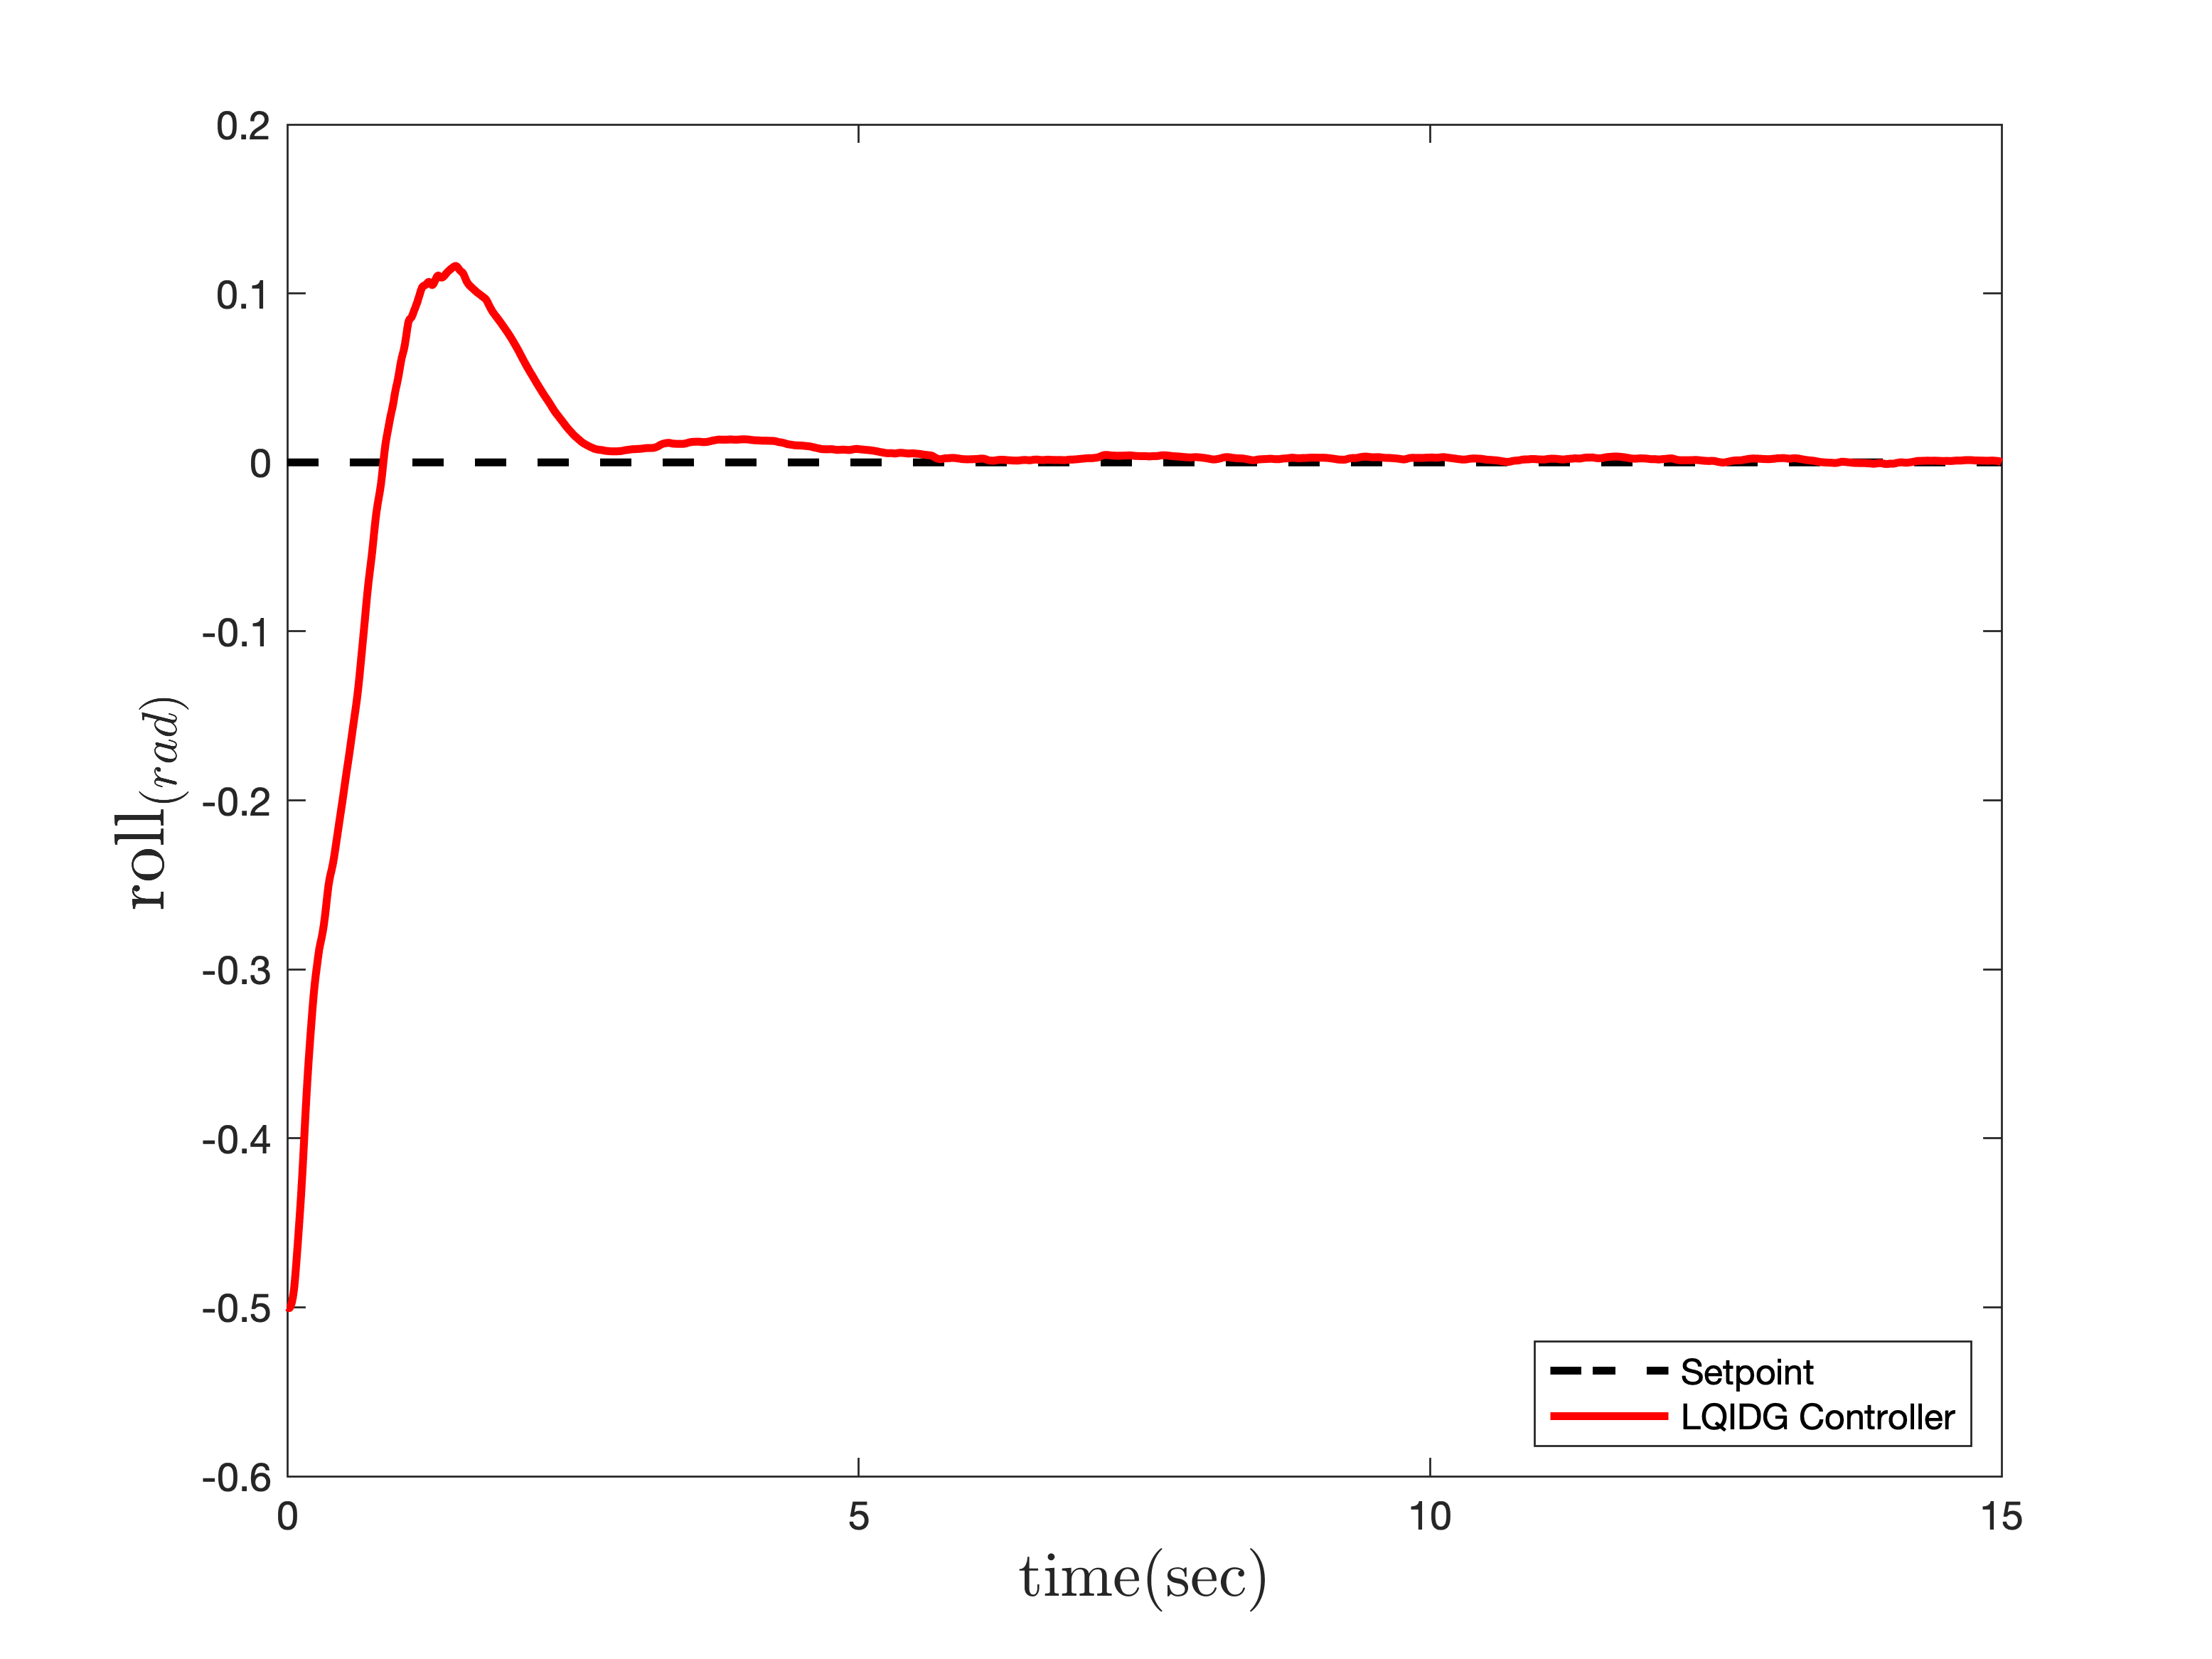
\includegraphics[width=.48\linewidth]{../Figures/MIL/LQIDG/MIMO/lqidg_roll.png}
%	}
%	\subfigure[تغییرات زاویه پیچ]{
%		\centering
%		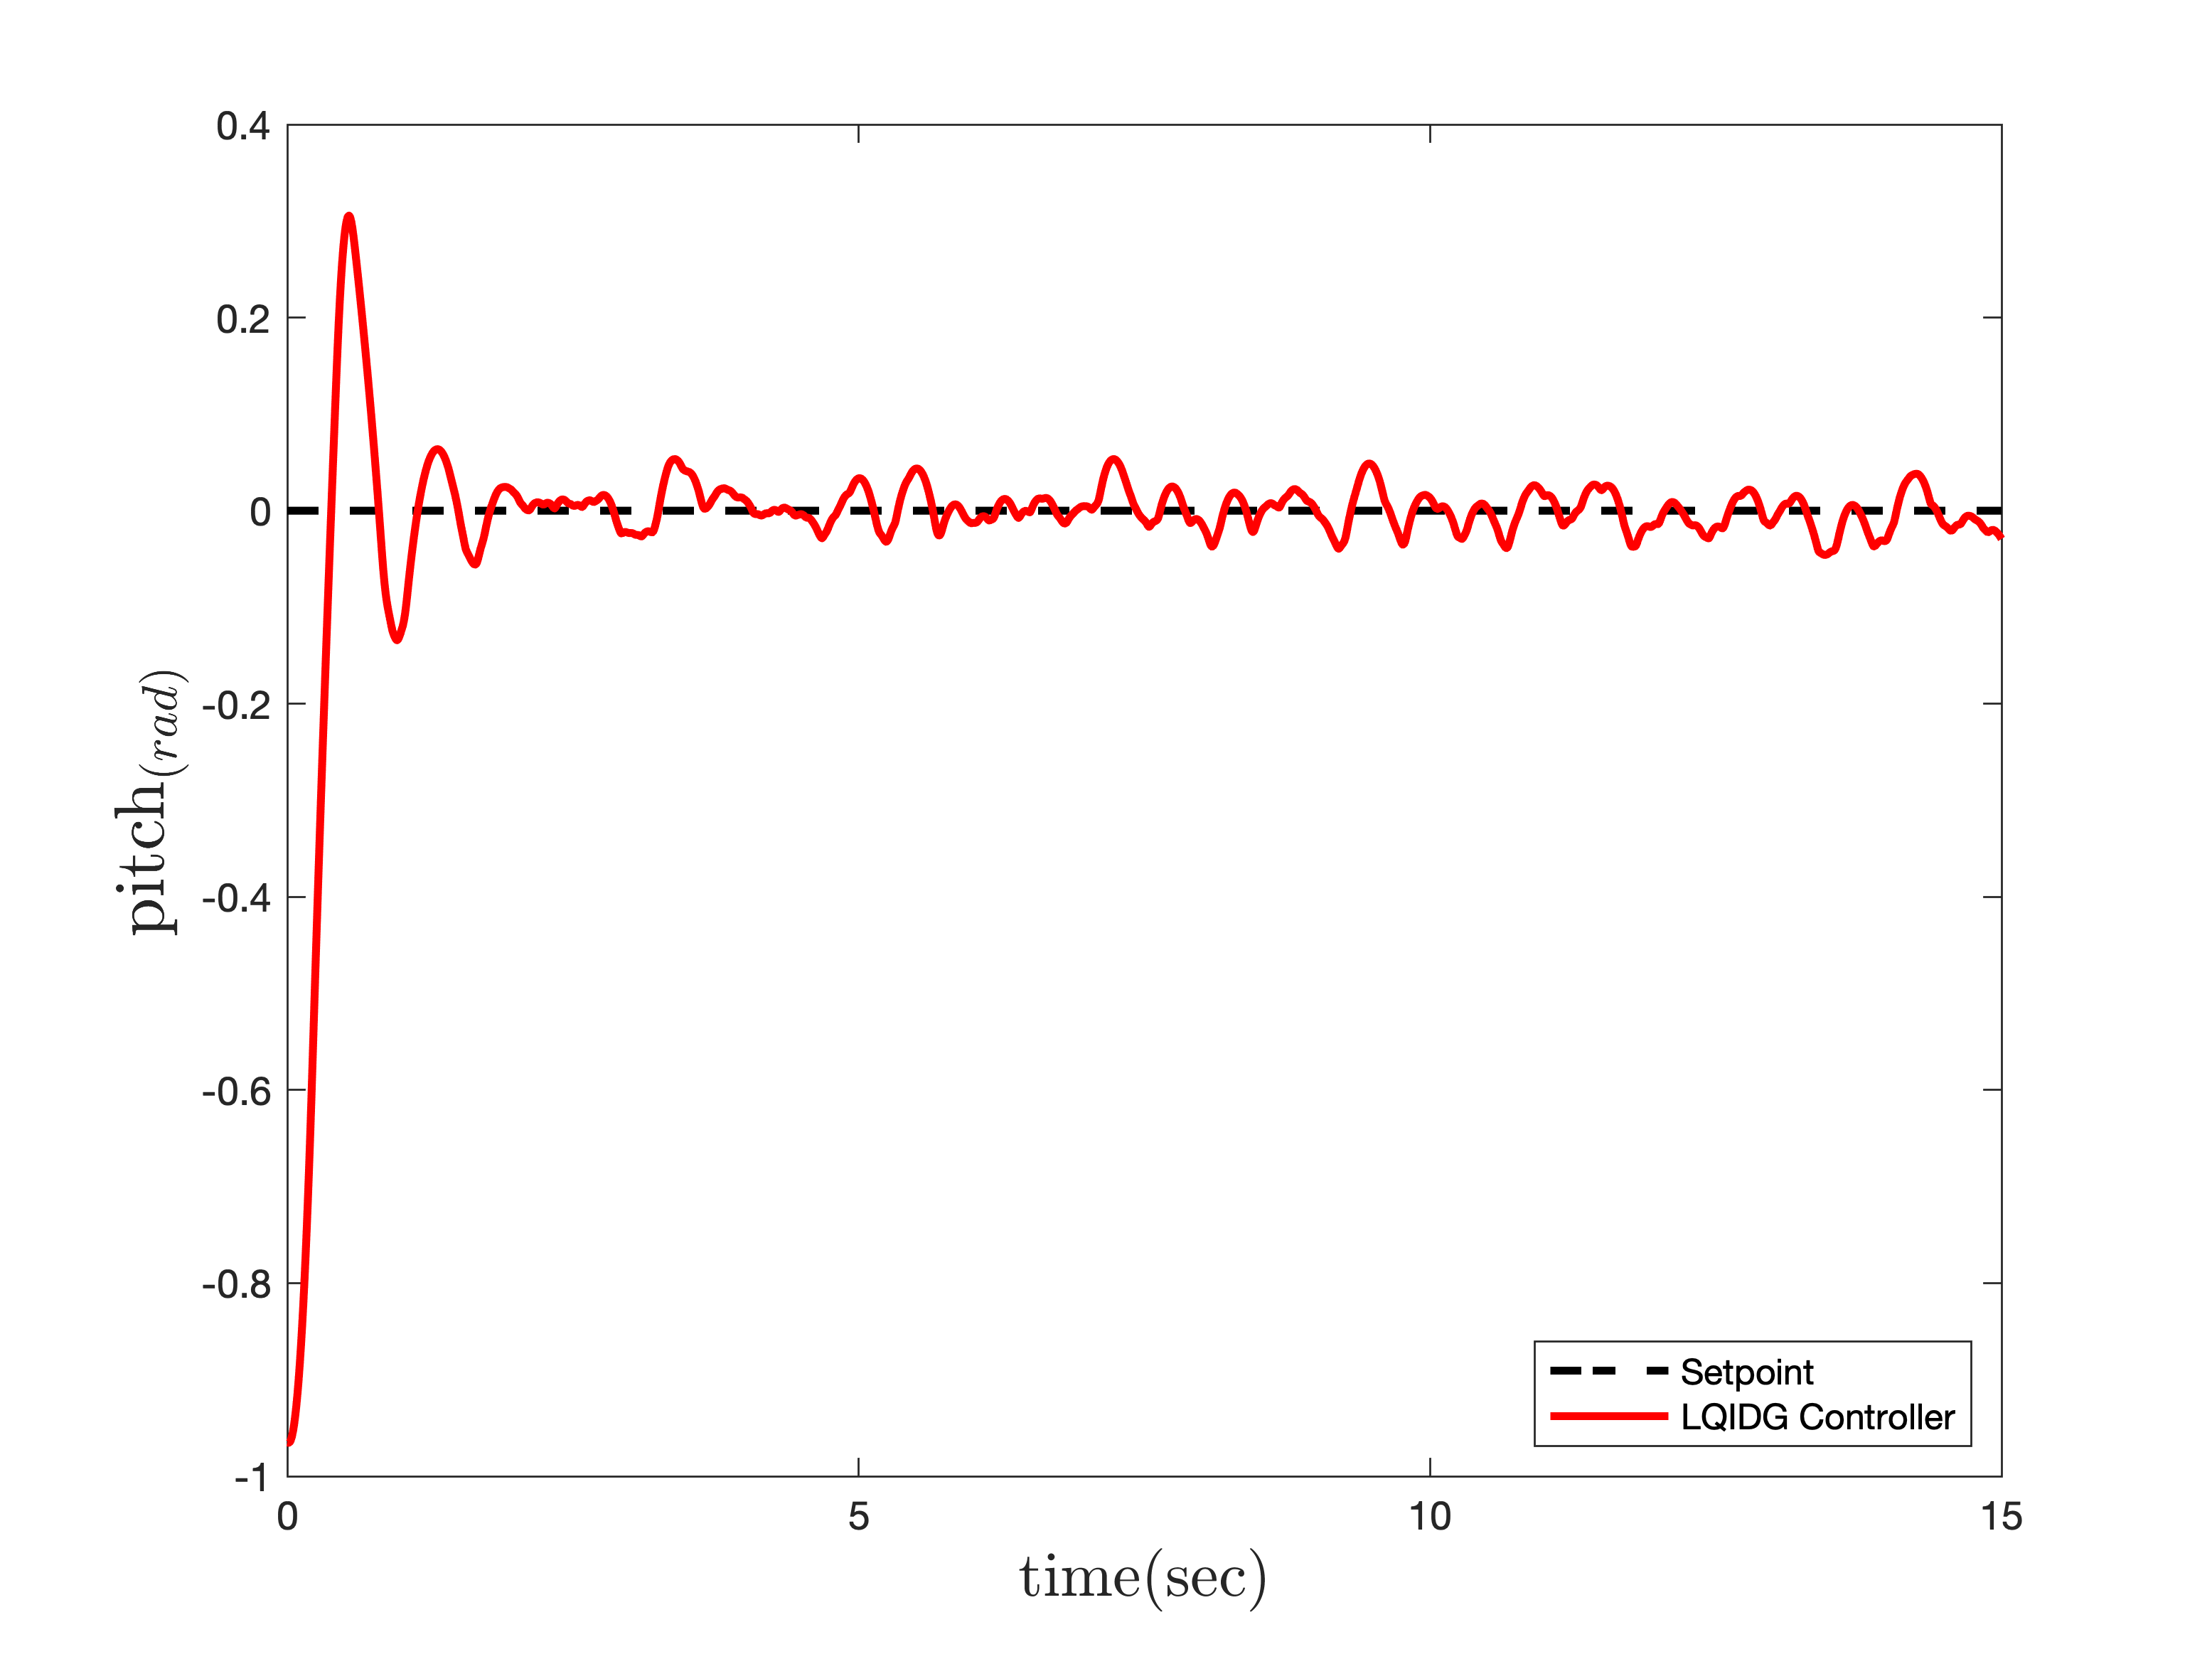
\includegraphics[width=.48\linewidth]{../Figures/MIL/LQIDG/MIMO/lqidg_pitch.png}
%	}
%	\subfigure[تغییرات زاویه یاو]{
%		\centering
%		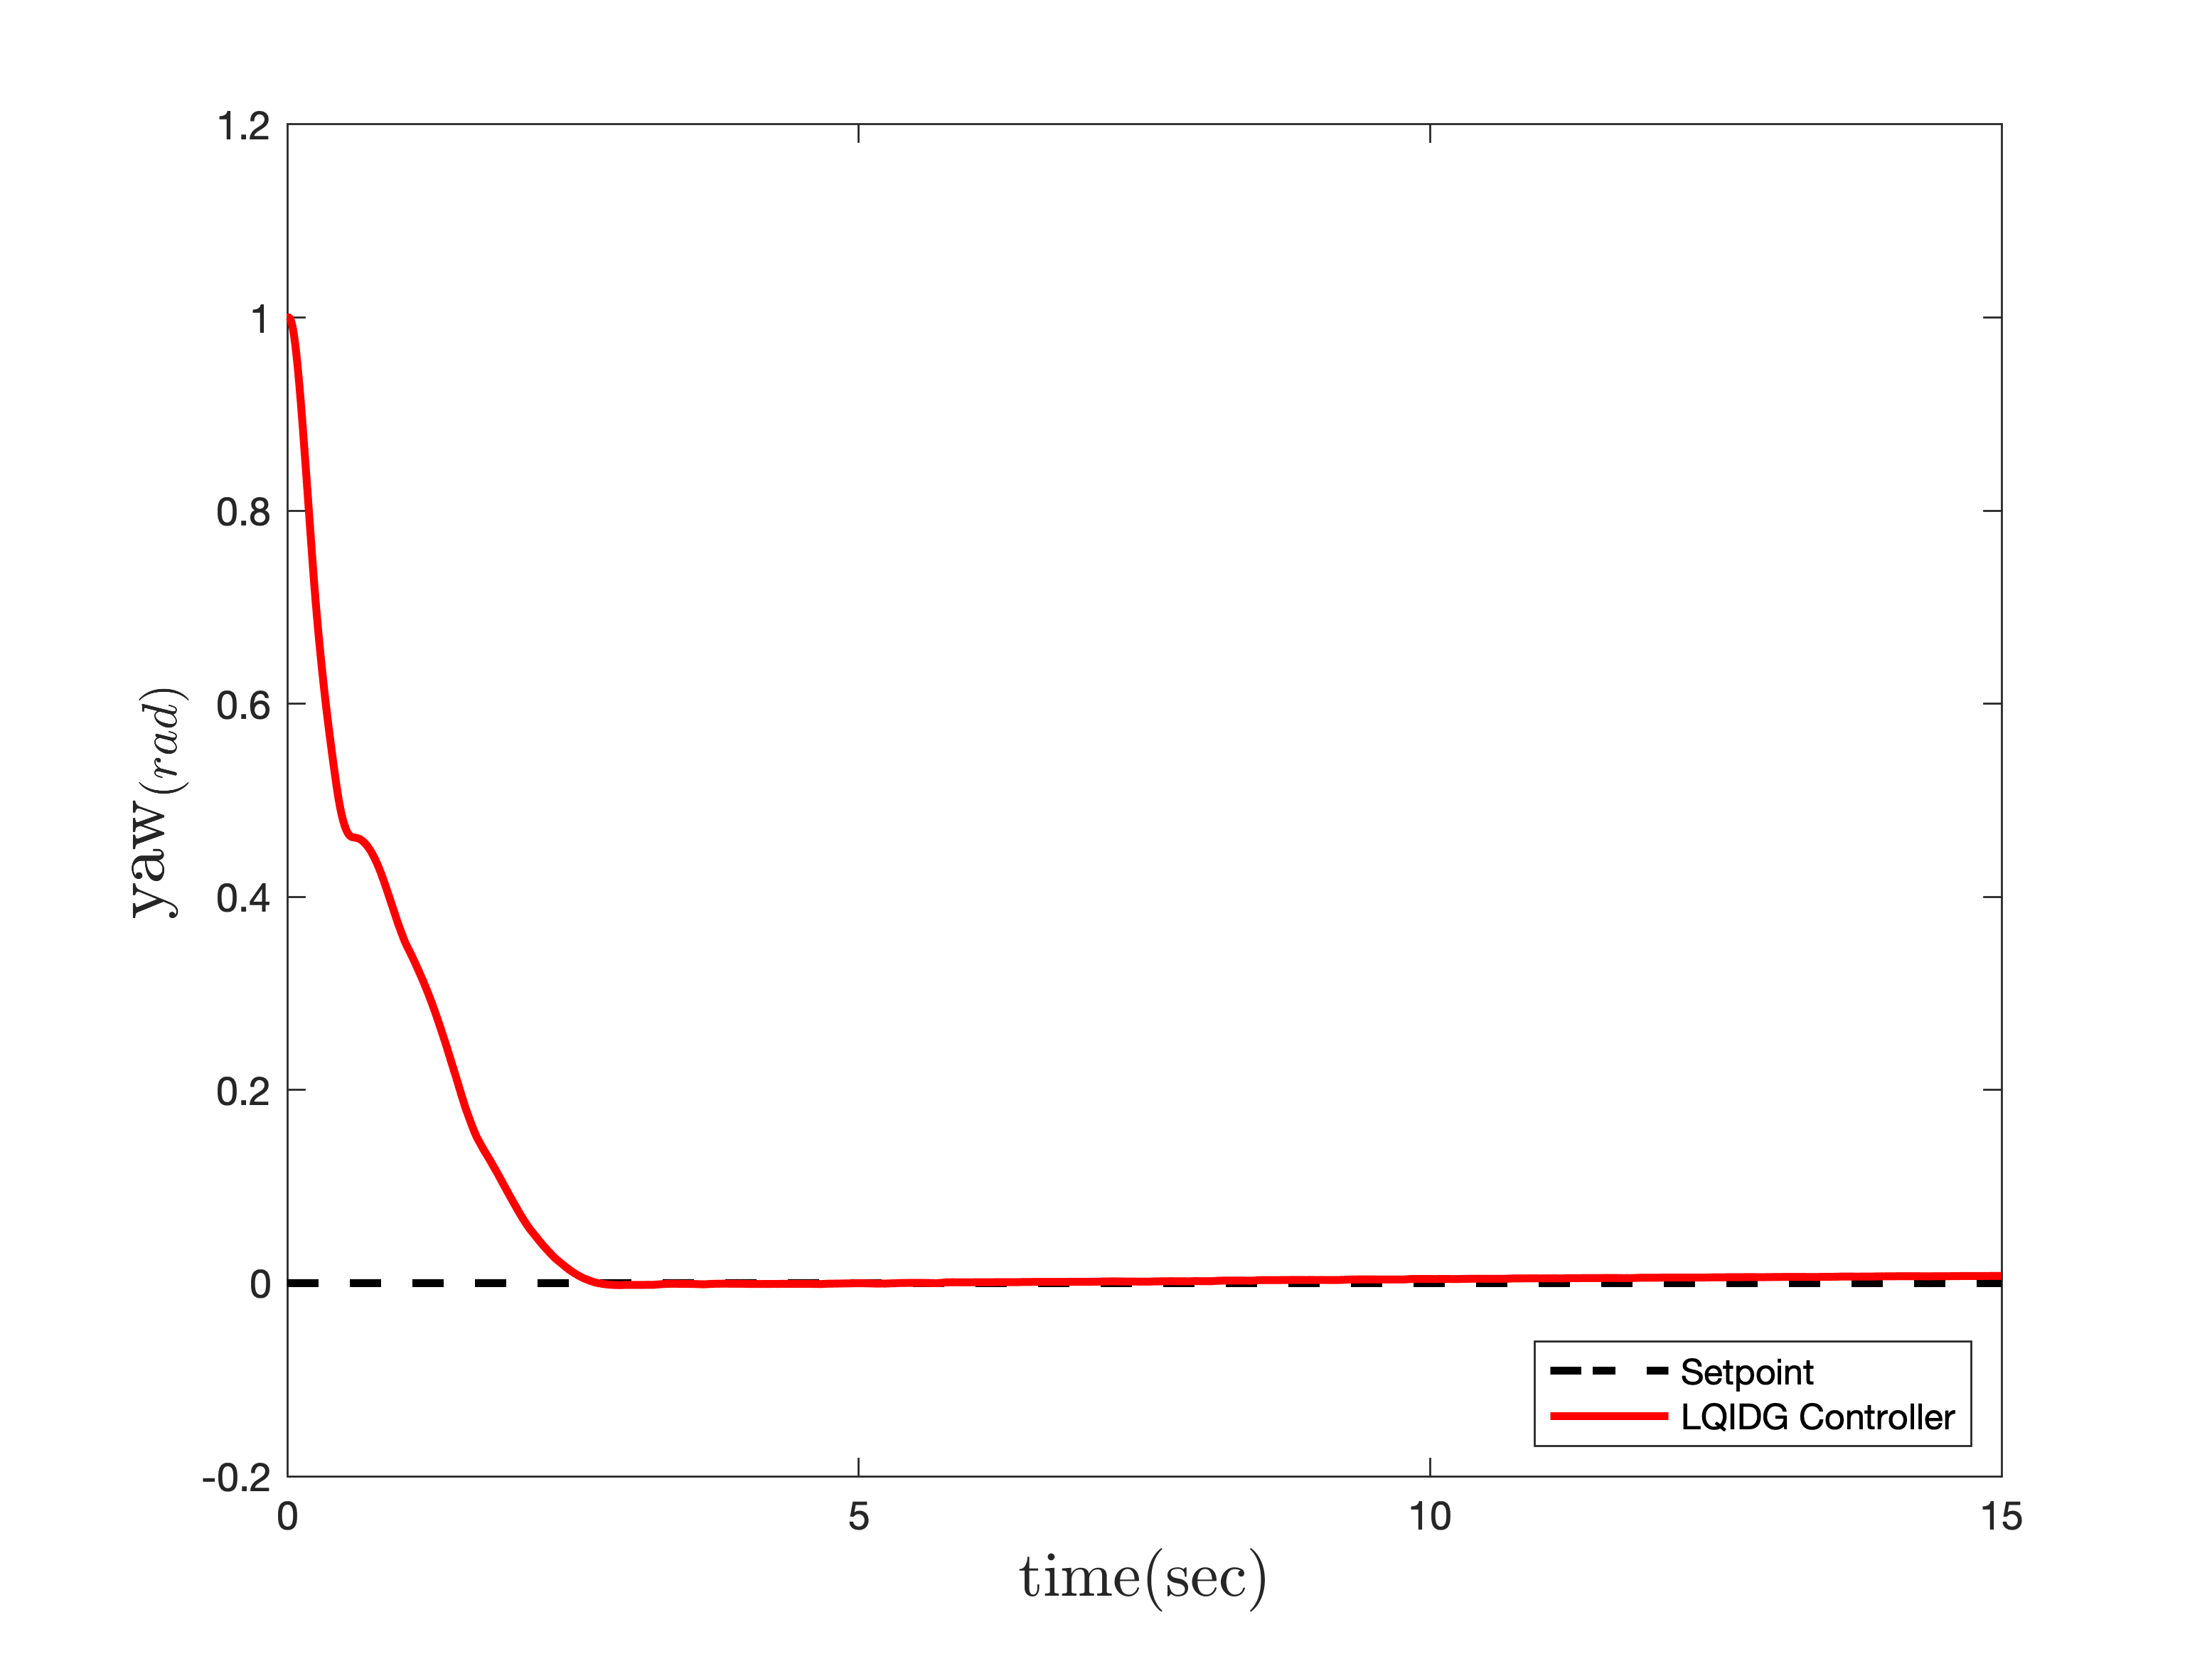
\includegraphics[width=.48\linewidth]{../Figures/MIL/LQIDG/MIMO/lqidg_yaw.png}
%	}
%	\caption{‫‪عملکرد کنترل‌کننده \lr{LQIDG} در کنترل وضعیت (تعقیب ورودی صفر)}
%	\label{lqidg_roll_pitch_yaw_fig_simulation_MIMO_noise}
%\end{figure}
%
%
%\begin{figure}[H]
%	\centering
%	\subfigure[موتور شماره یک]{
%		\centering
%		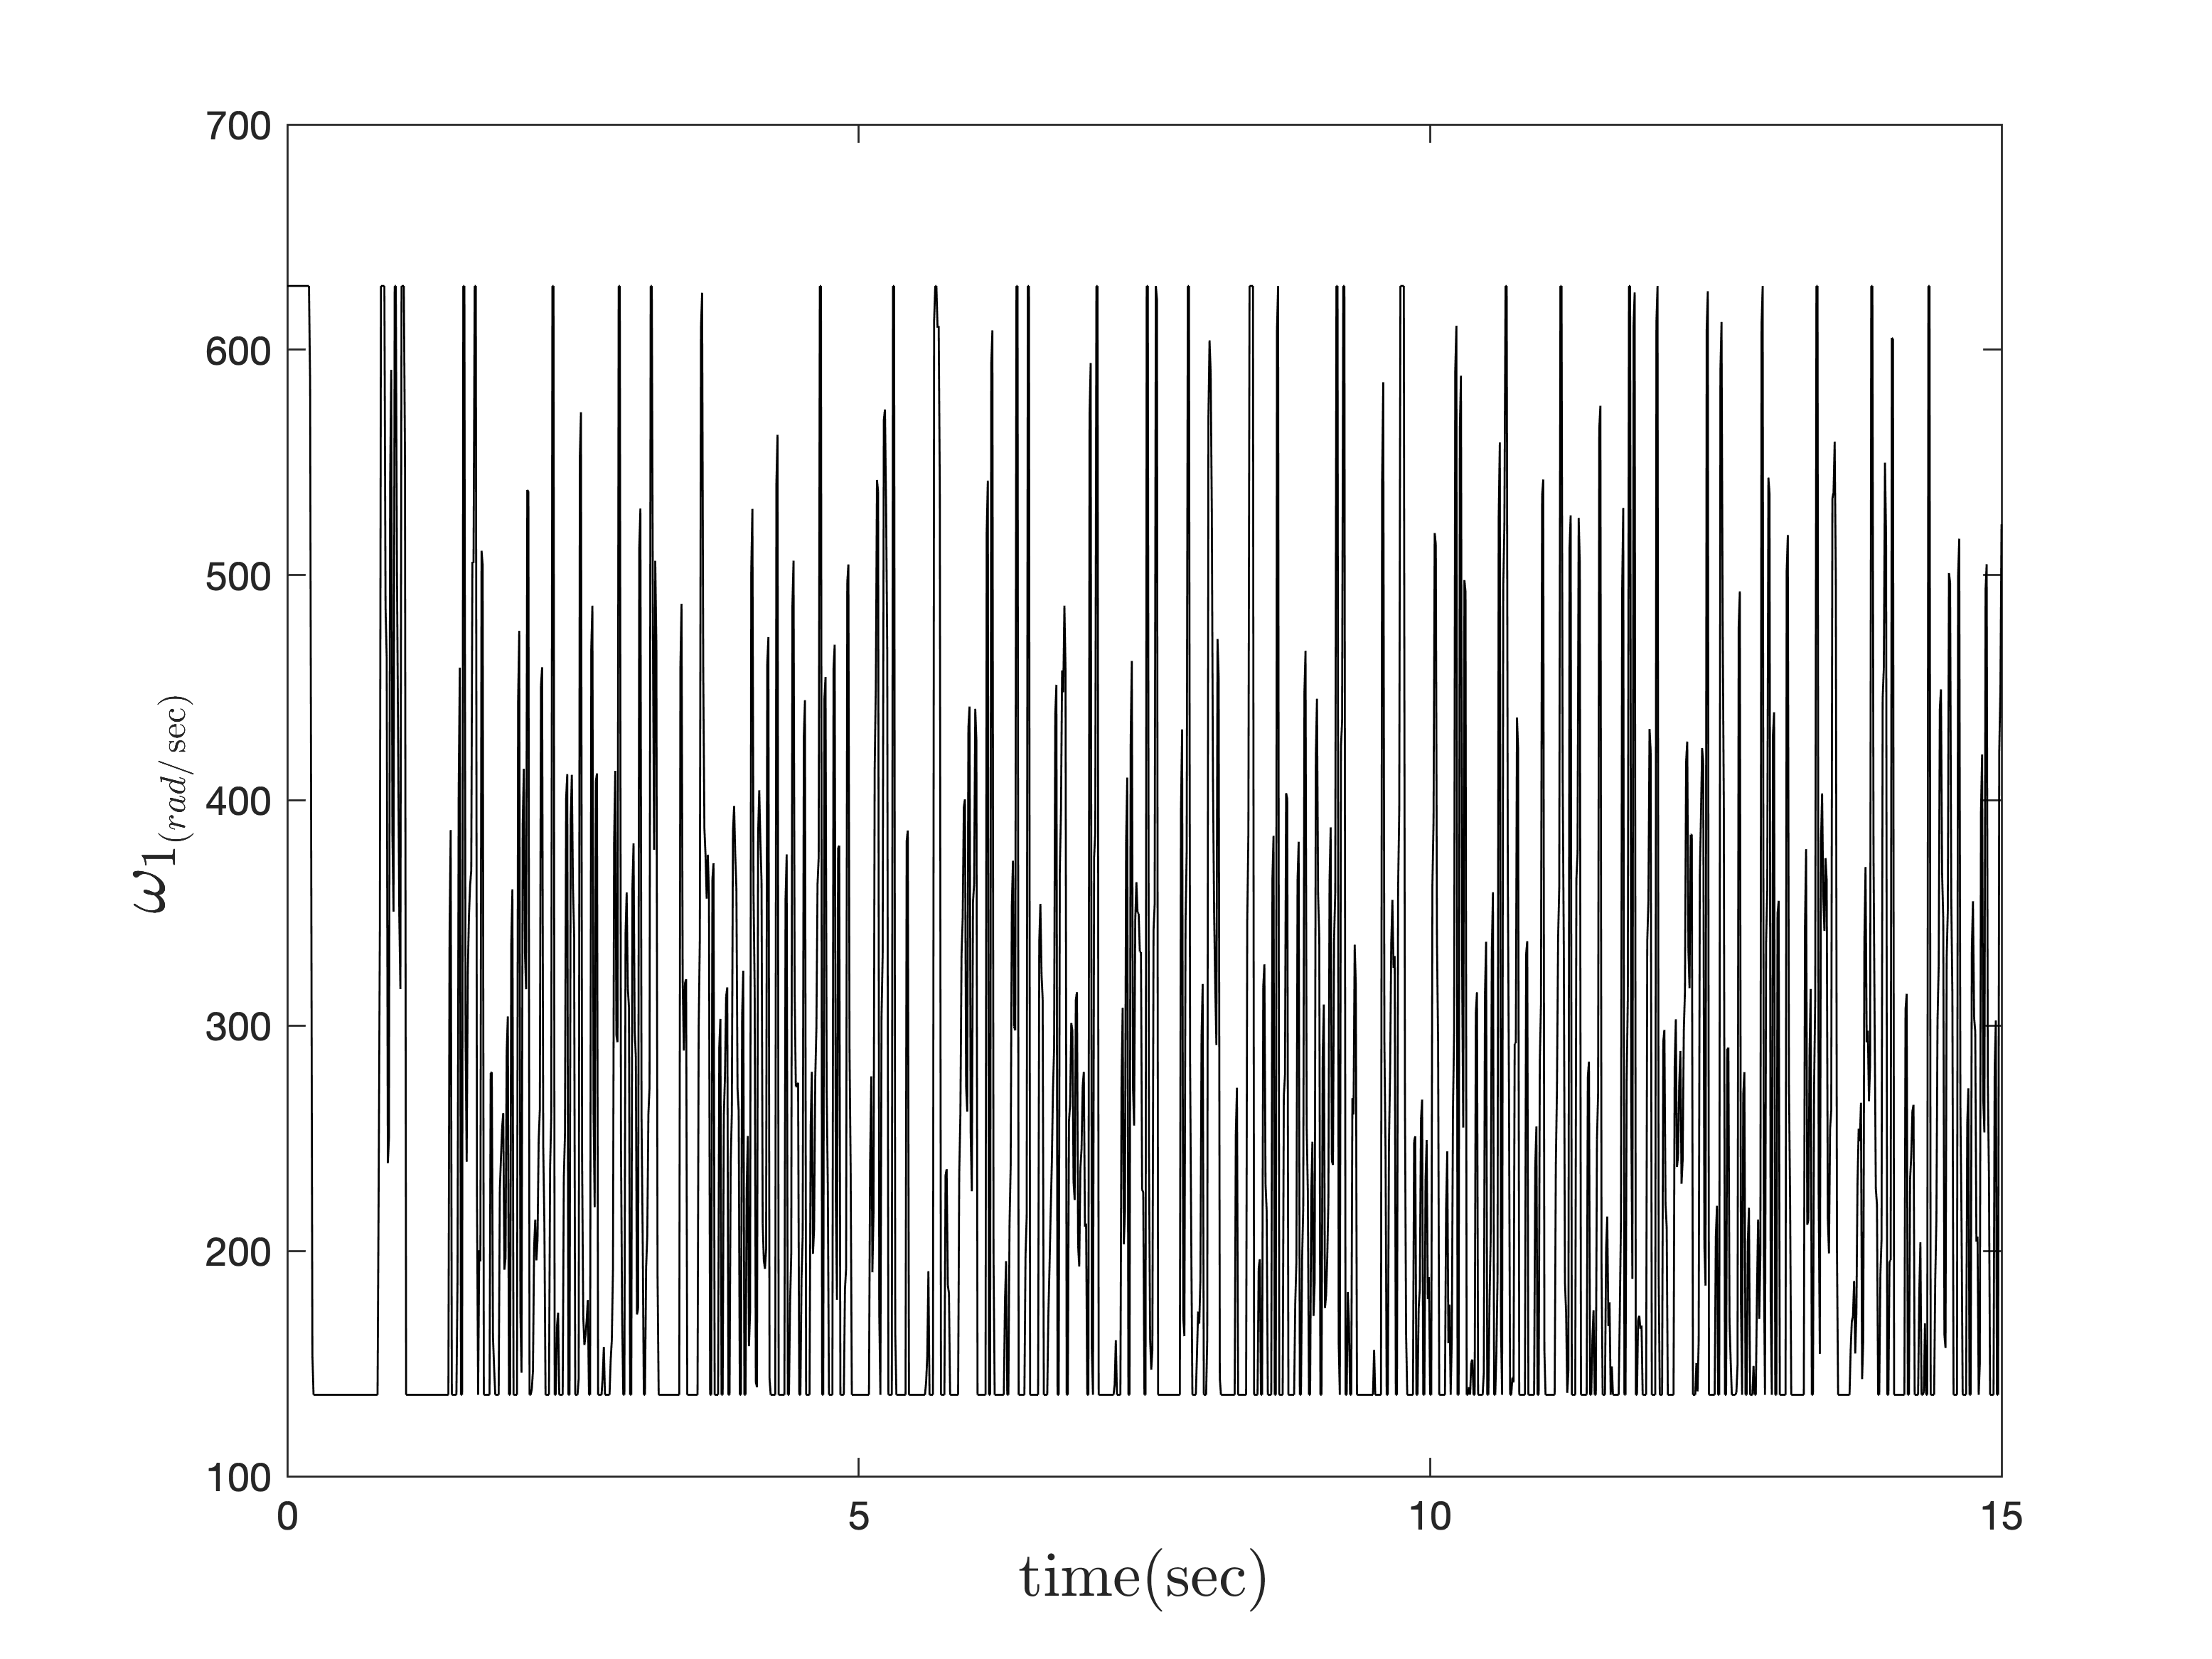
\includegraphics[width=.45\linewidth]{../Figures/MIL/LQIDG/MIMO/lqidg_roll_pitch_omega_1.png}
%	}
%	\subfigure[موتور شماره دو]{
%		\centering
%		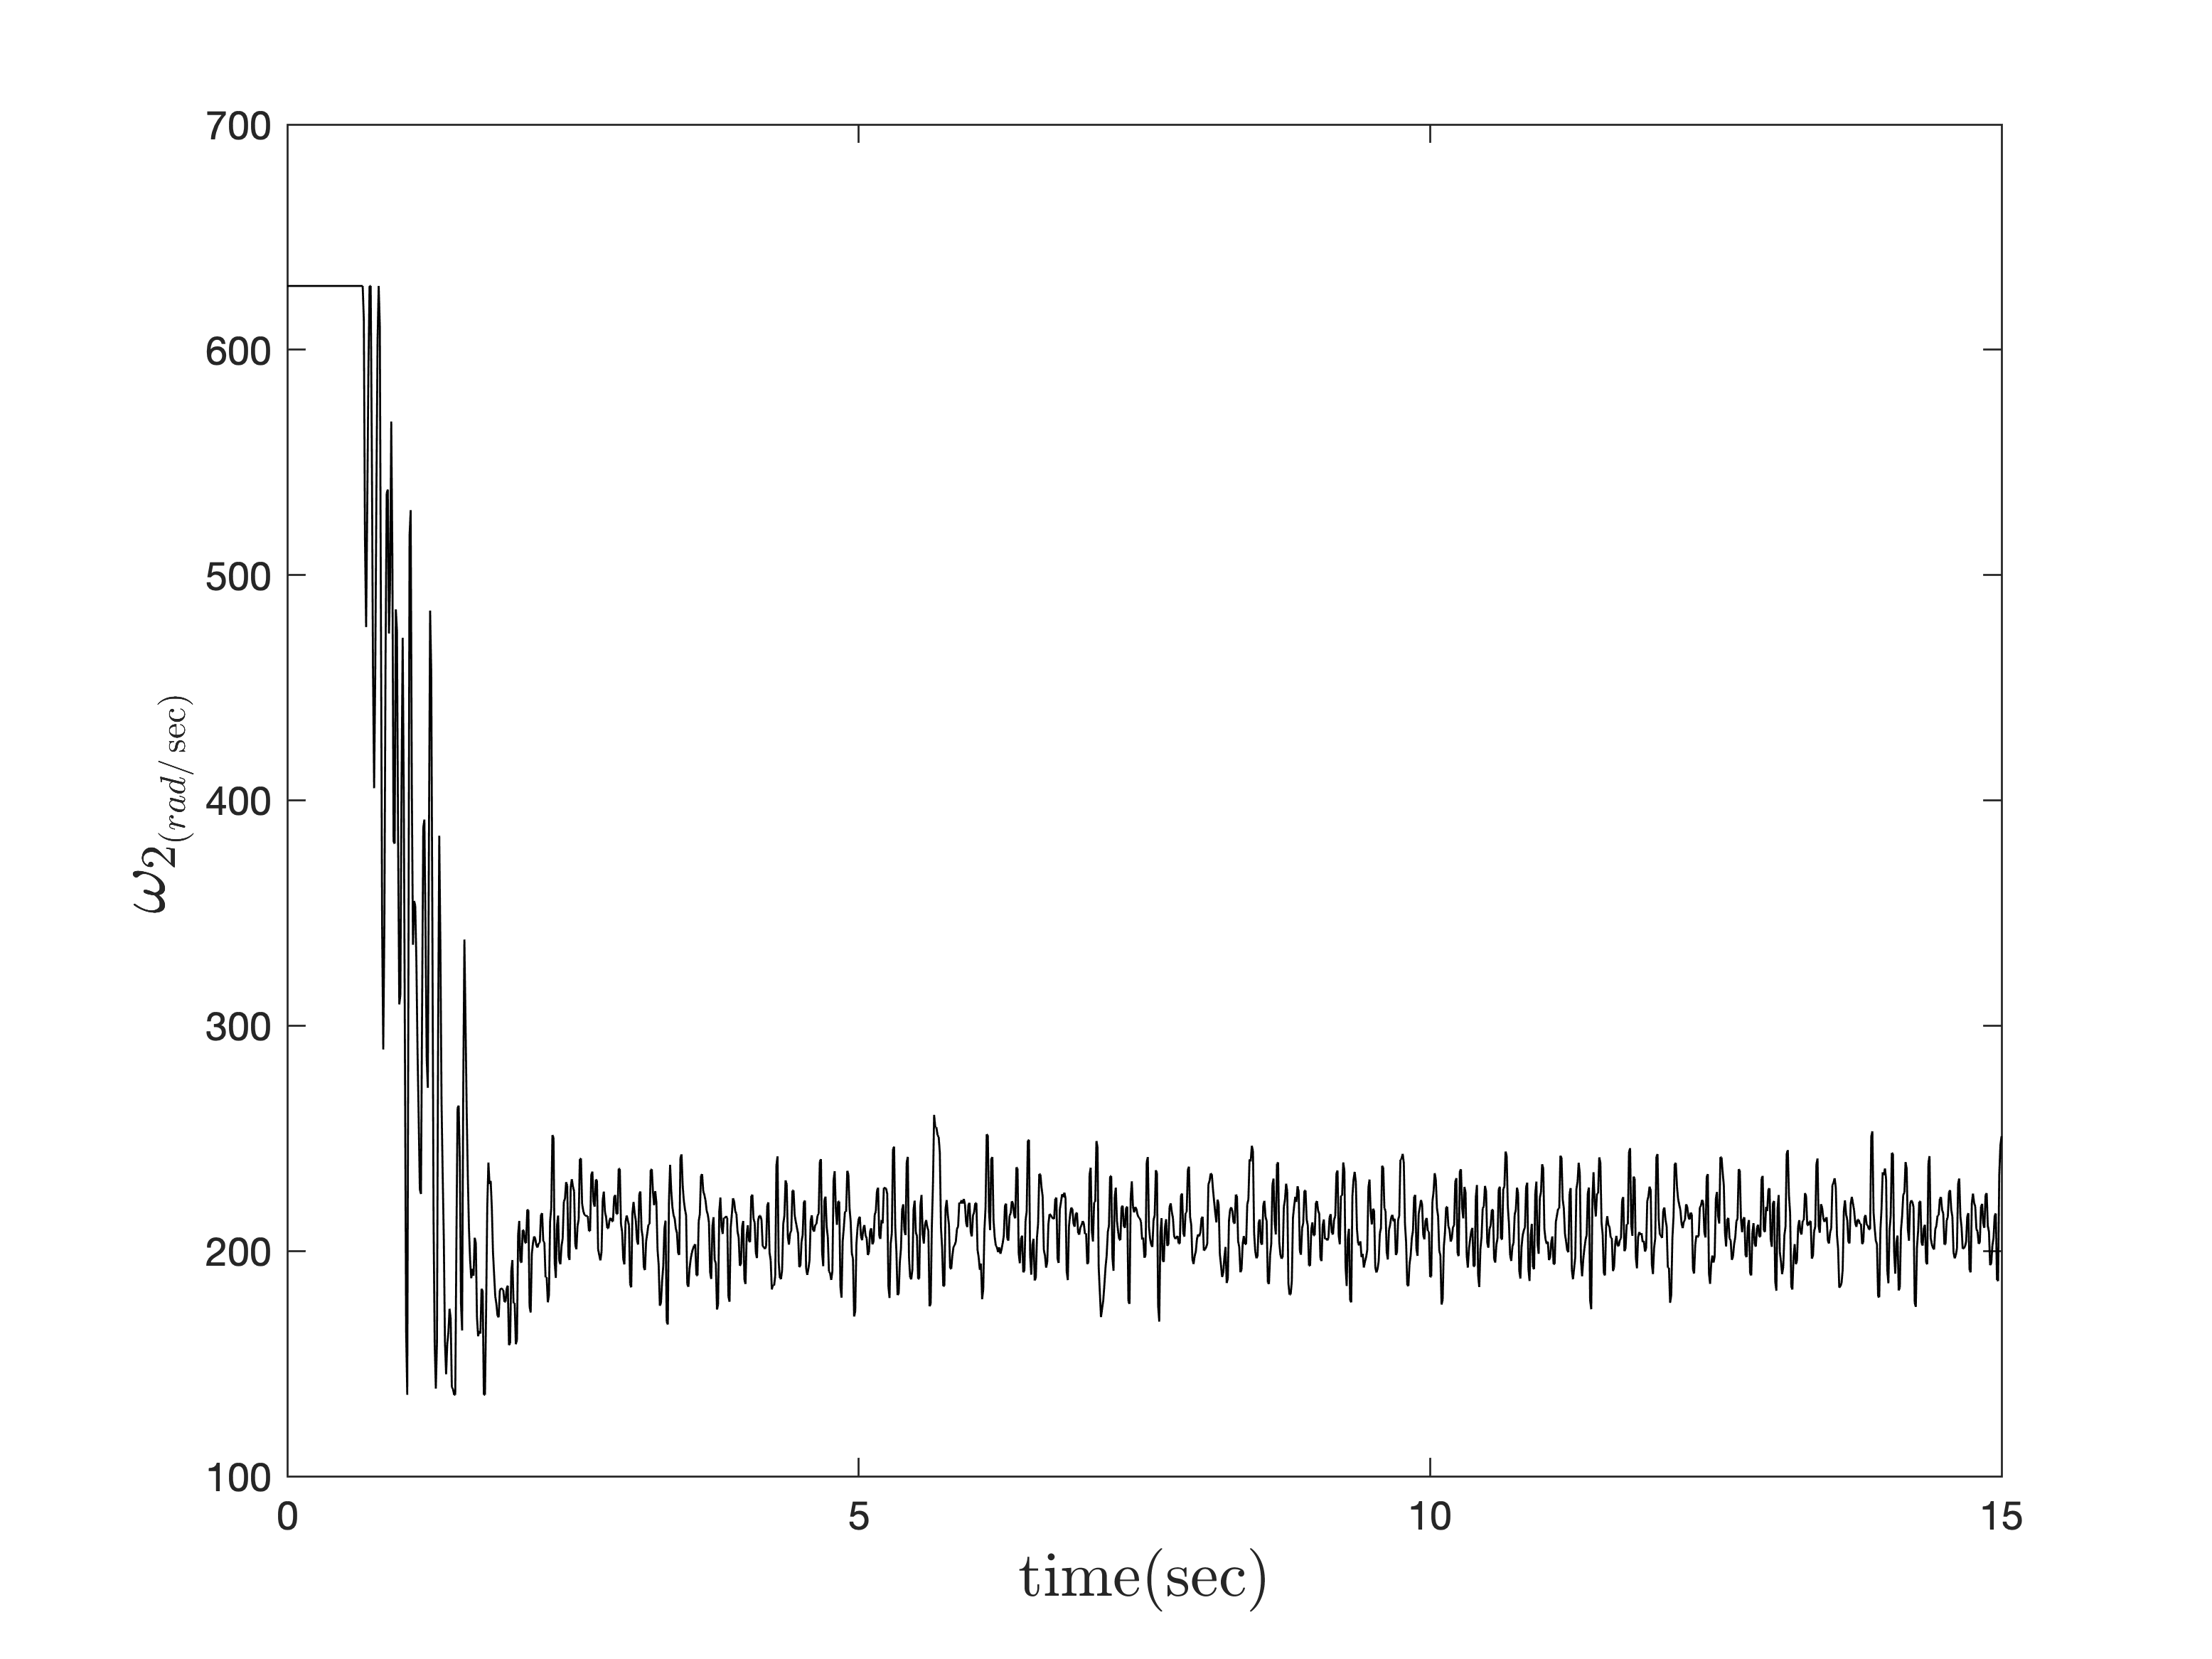
\includegraphics[width=.45\linewidth]{../Figures/MIL/LQIDG/MIMO/lqidg_roll_pitch_omega_2.png}
%	}
%	\subfigure[موتور شماره سه]{
%		\centering
%		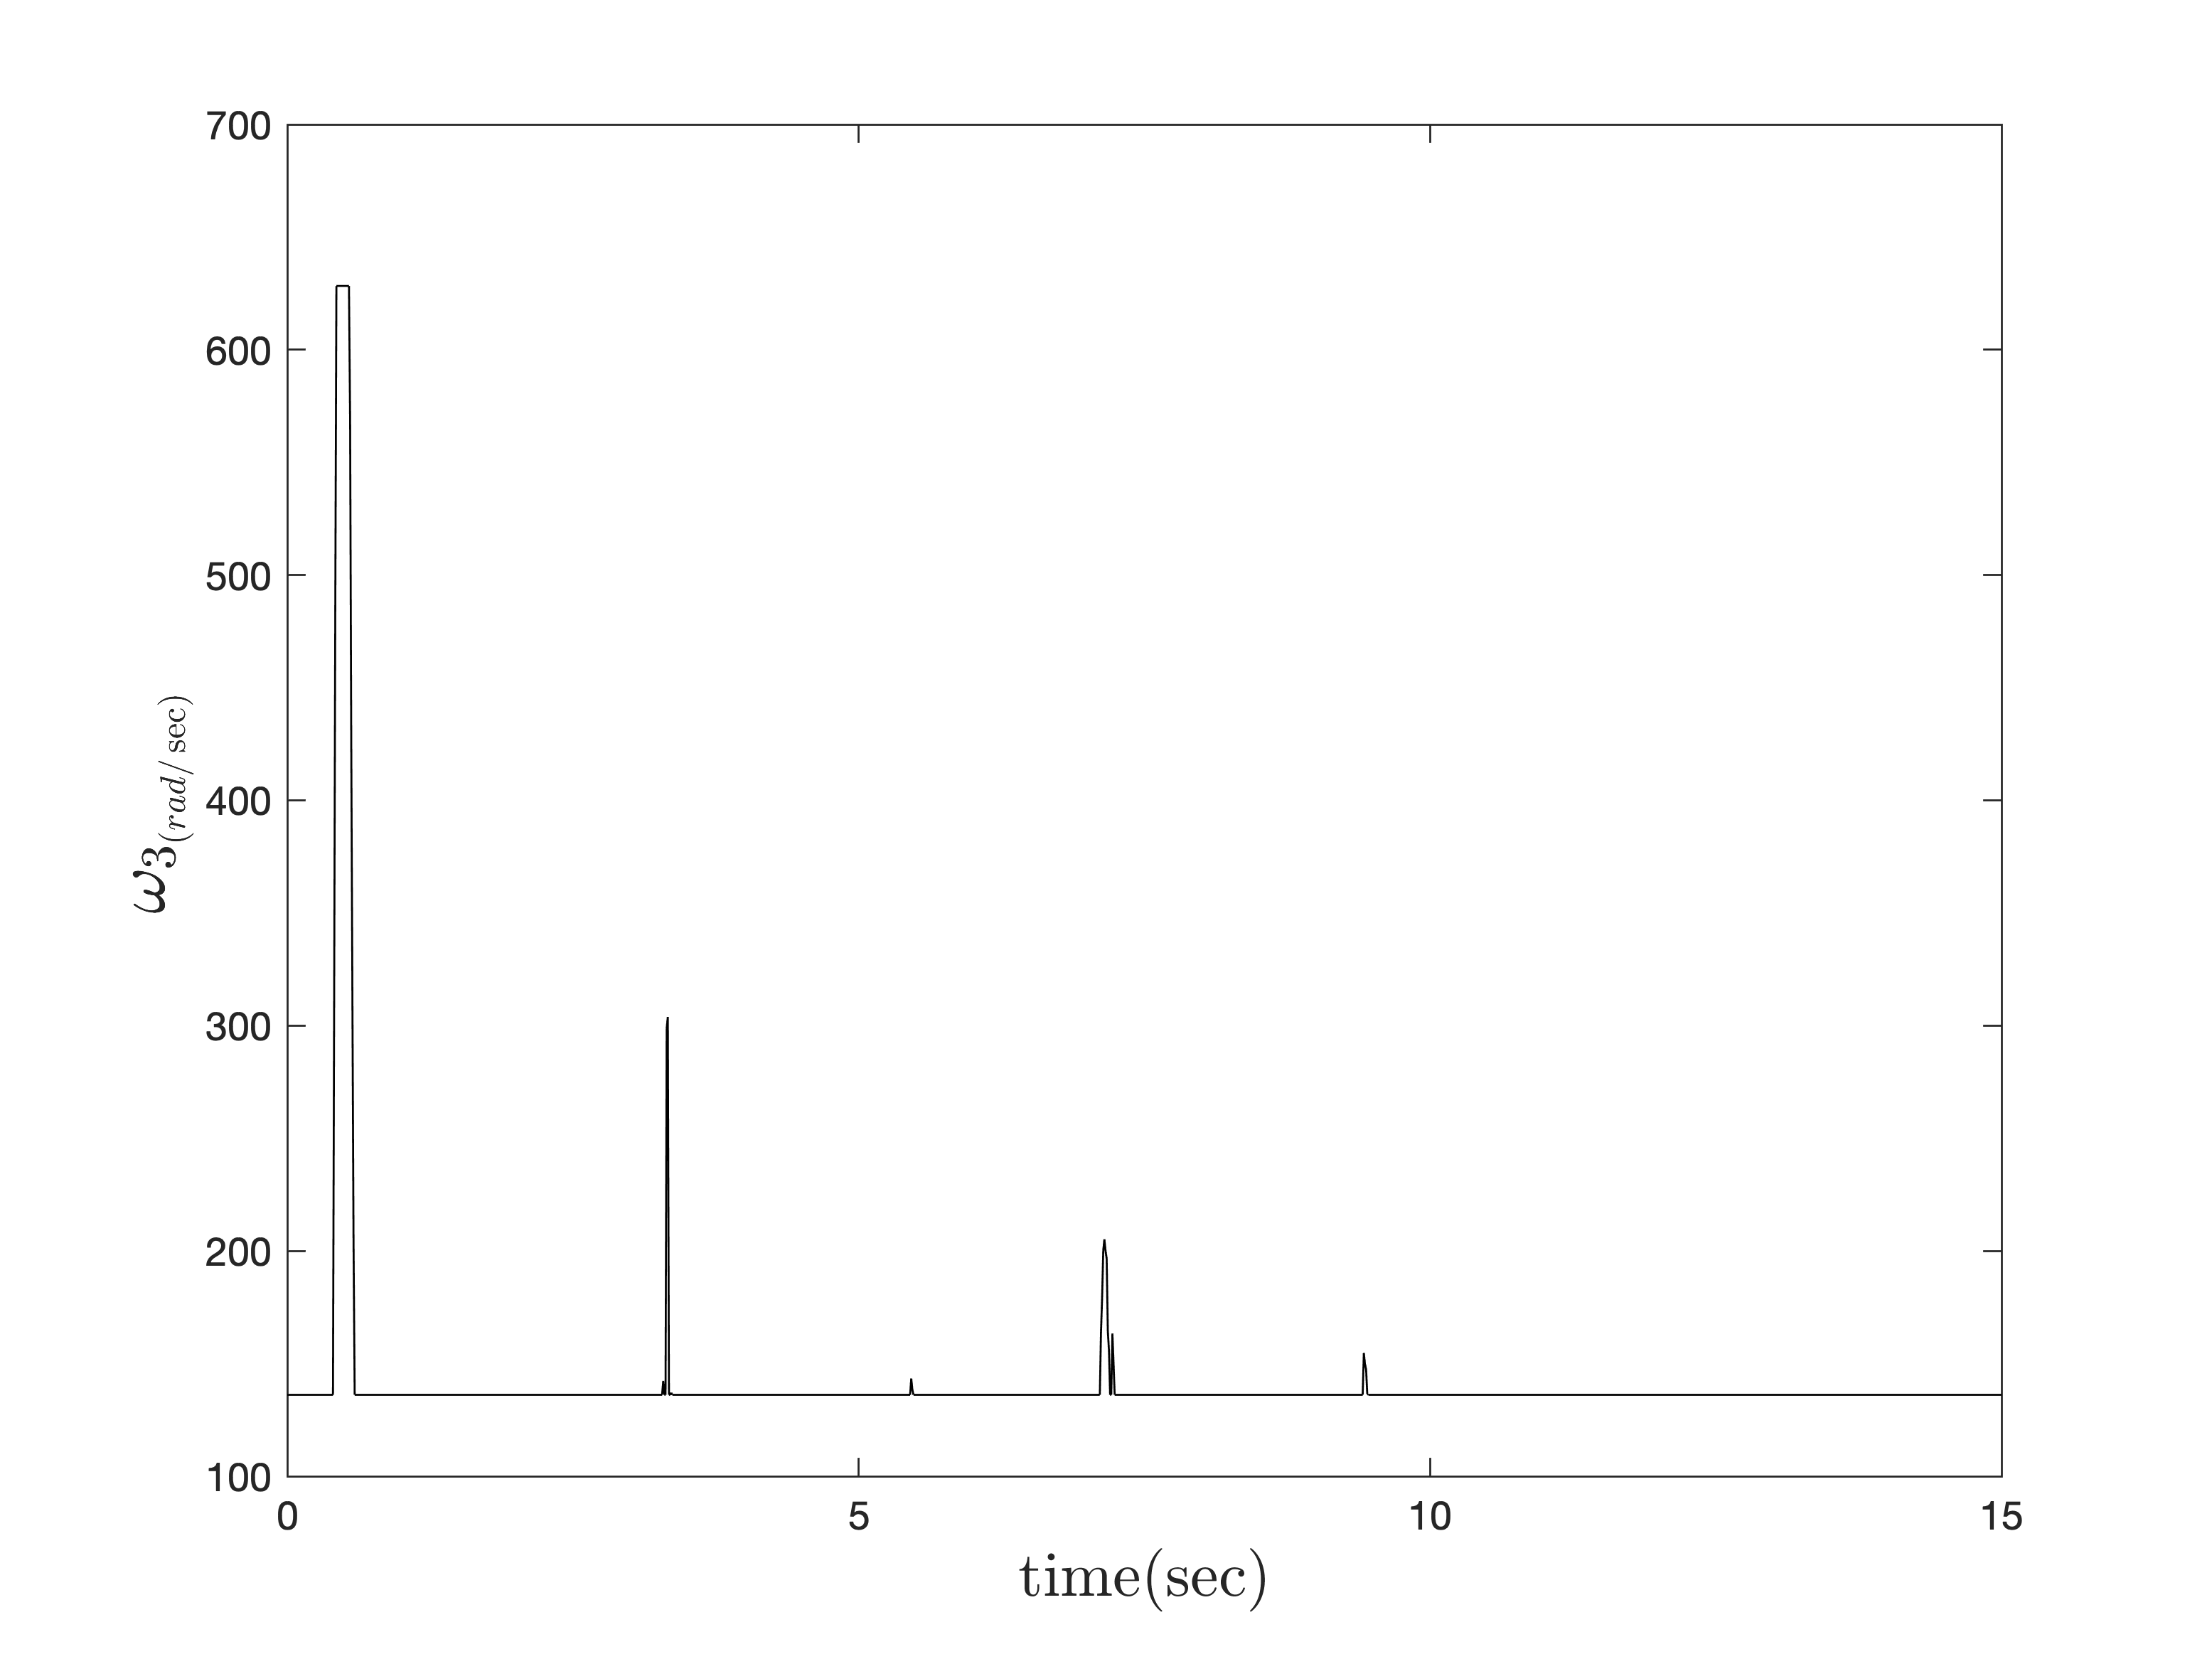
\includegraphics[width=.45\linewidth]{../Figures/MIL/LQIDG/MIMO/lqidg_roll_pitch_omega_3.png}
%	}
%	\subfigure[موتور شماره چهار]{
%		\centering
%		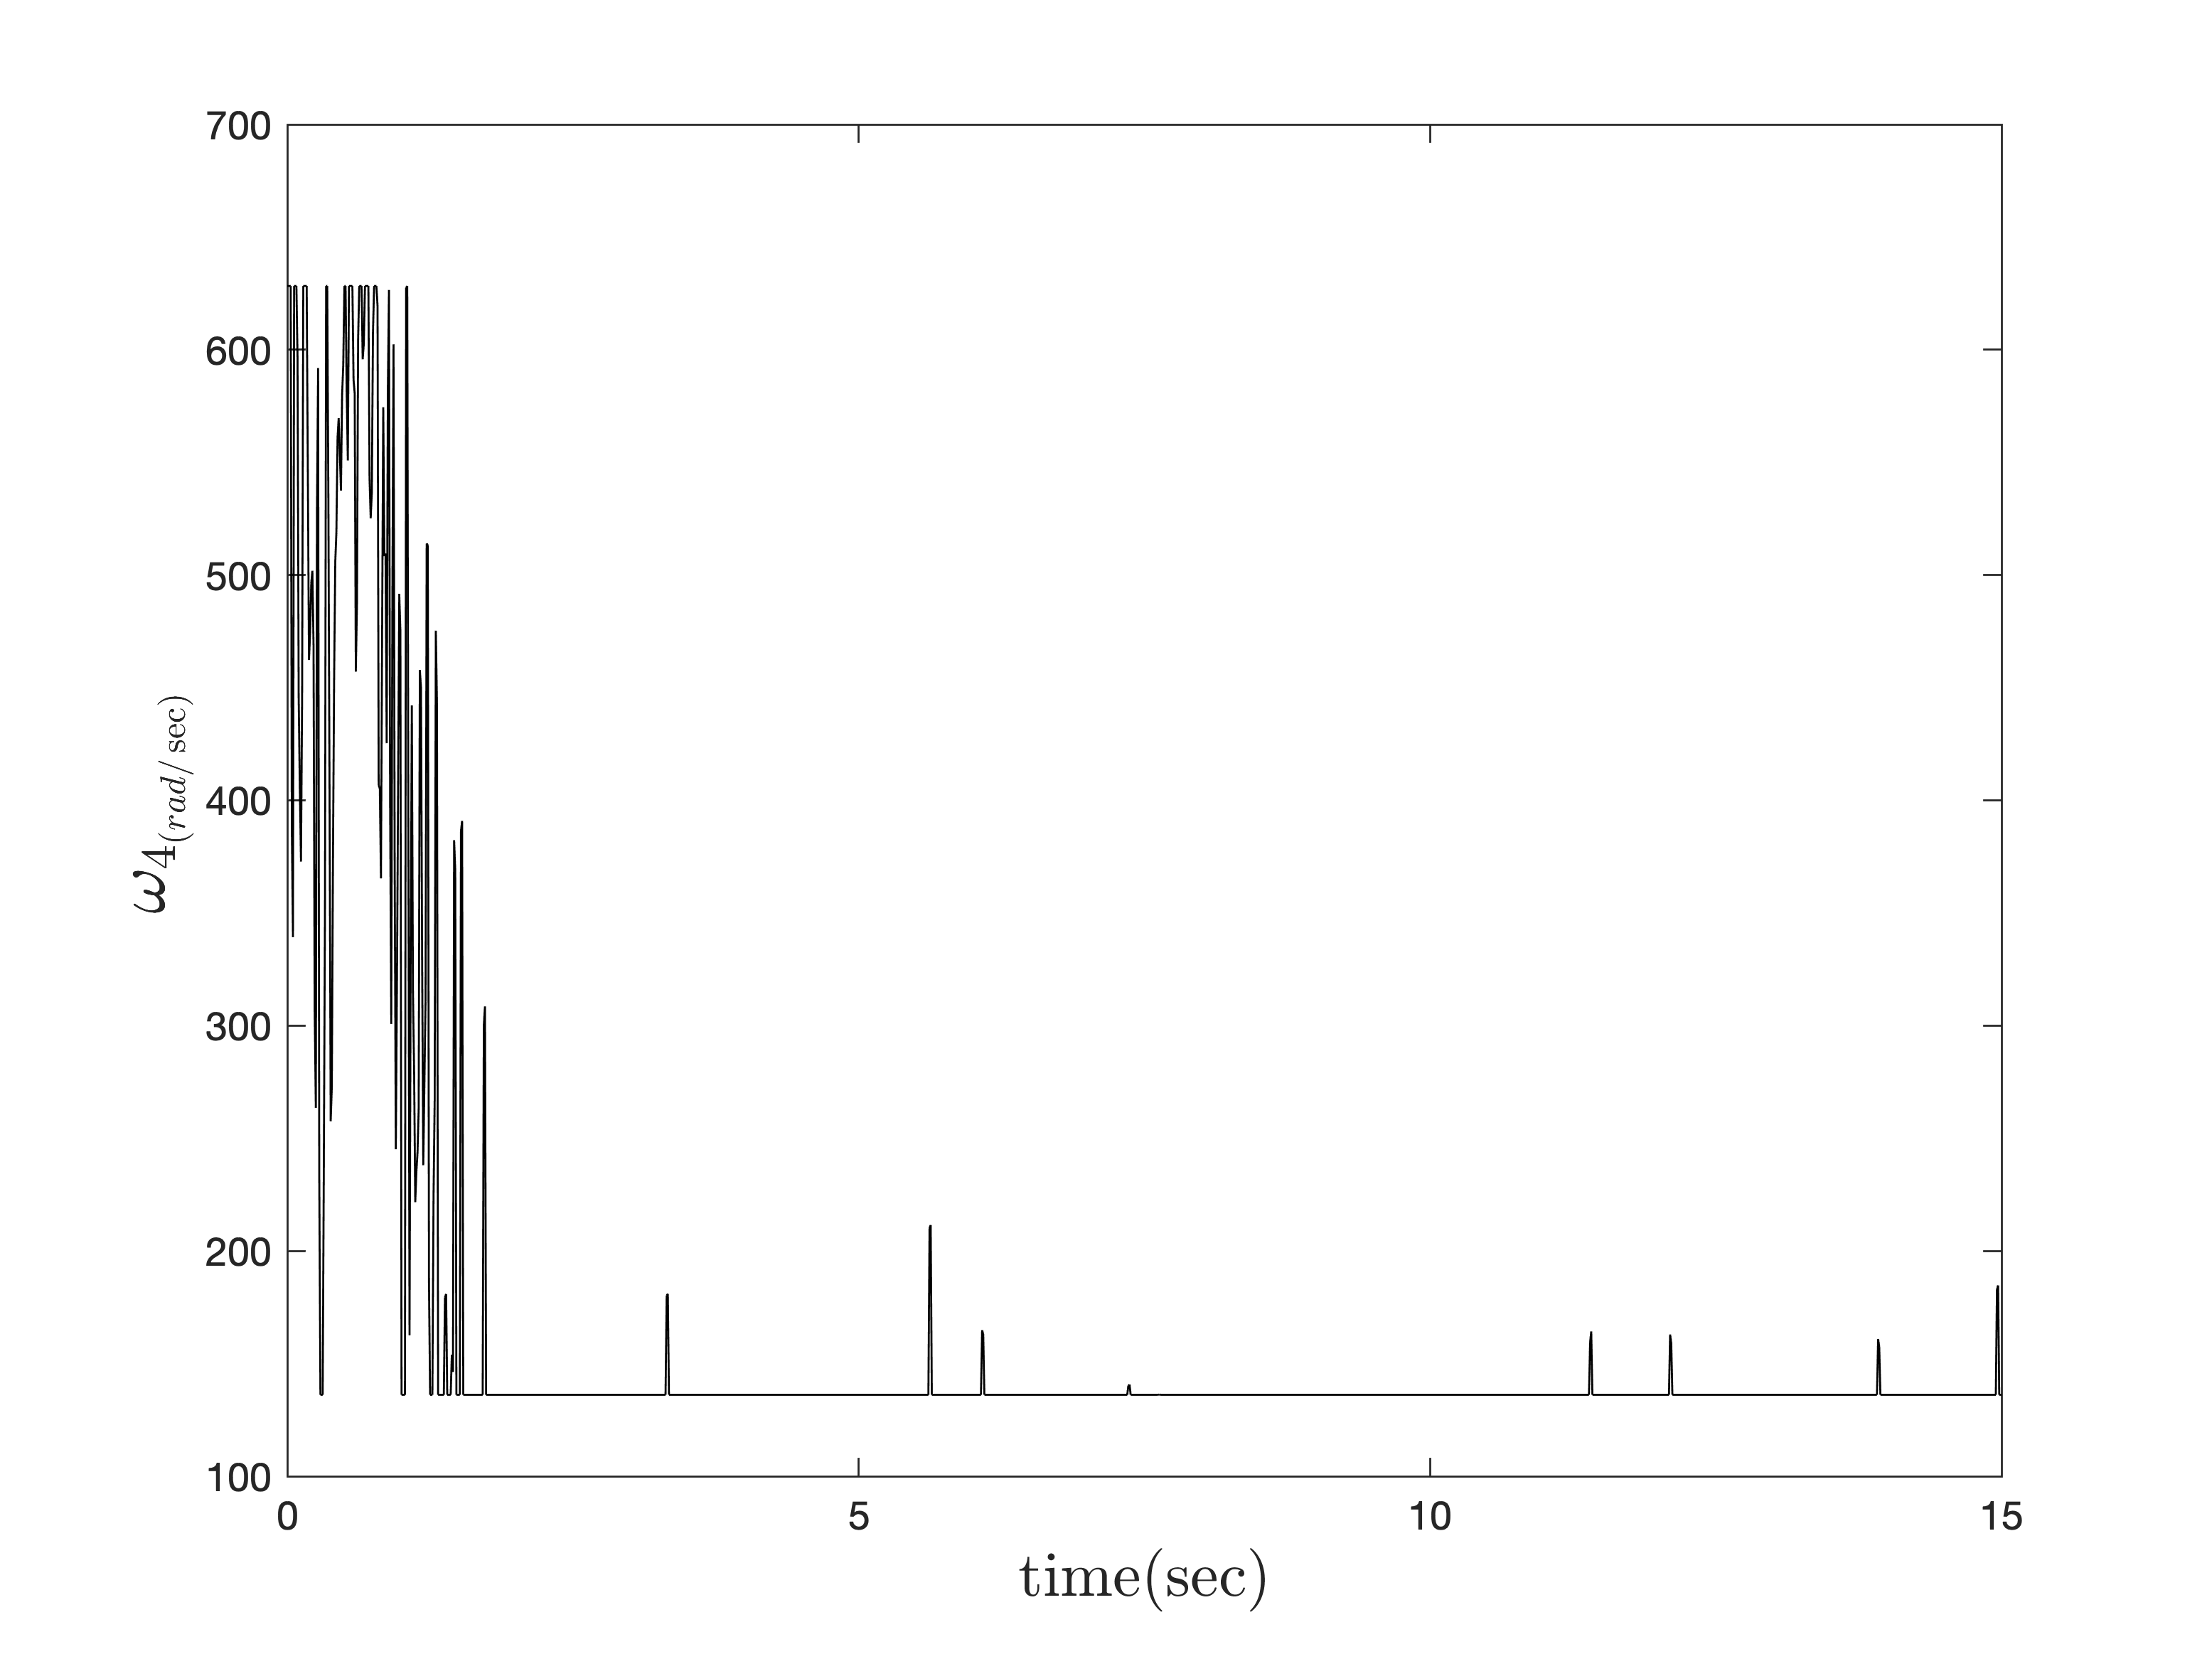
\includegraphics[width=.45\linewidth]{../Figures/MIL/LQIDG/MIMO/lqidg_roll_pitch_omega_4.png}
%	}
%	\caption{‫‪فرمان کنترلی موتورها در کنترل وضعیت (تعقیب ورودی صفر)}
%\end{figure}
%\بدون‌تورفتگی همانطور که از شکل
%\ref{lqidg_roll_pitch_yaw_fig_simulation_MIMO_noise}
%مشخص است، عملکرد کنترل‌کننده \lr{LQDG} در برابر نویز اندازه‌گیری خوب است و خروجی نوسان ندارد.
%
%\subsubsection{شبیه‌سازی کنترل‌کننده به‌صورت سه کانال تک ورودی}
%\begin{figure}[H]
%	\centering
%	\begin{subfigure}[H]
%		\centering
%		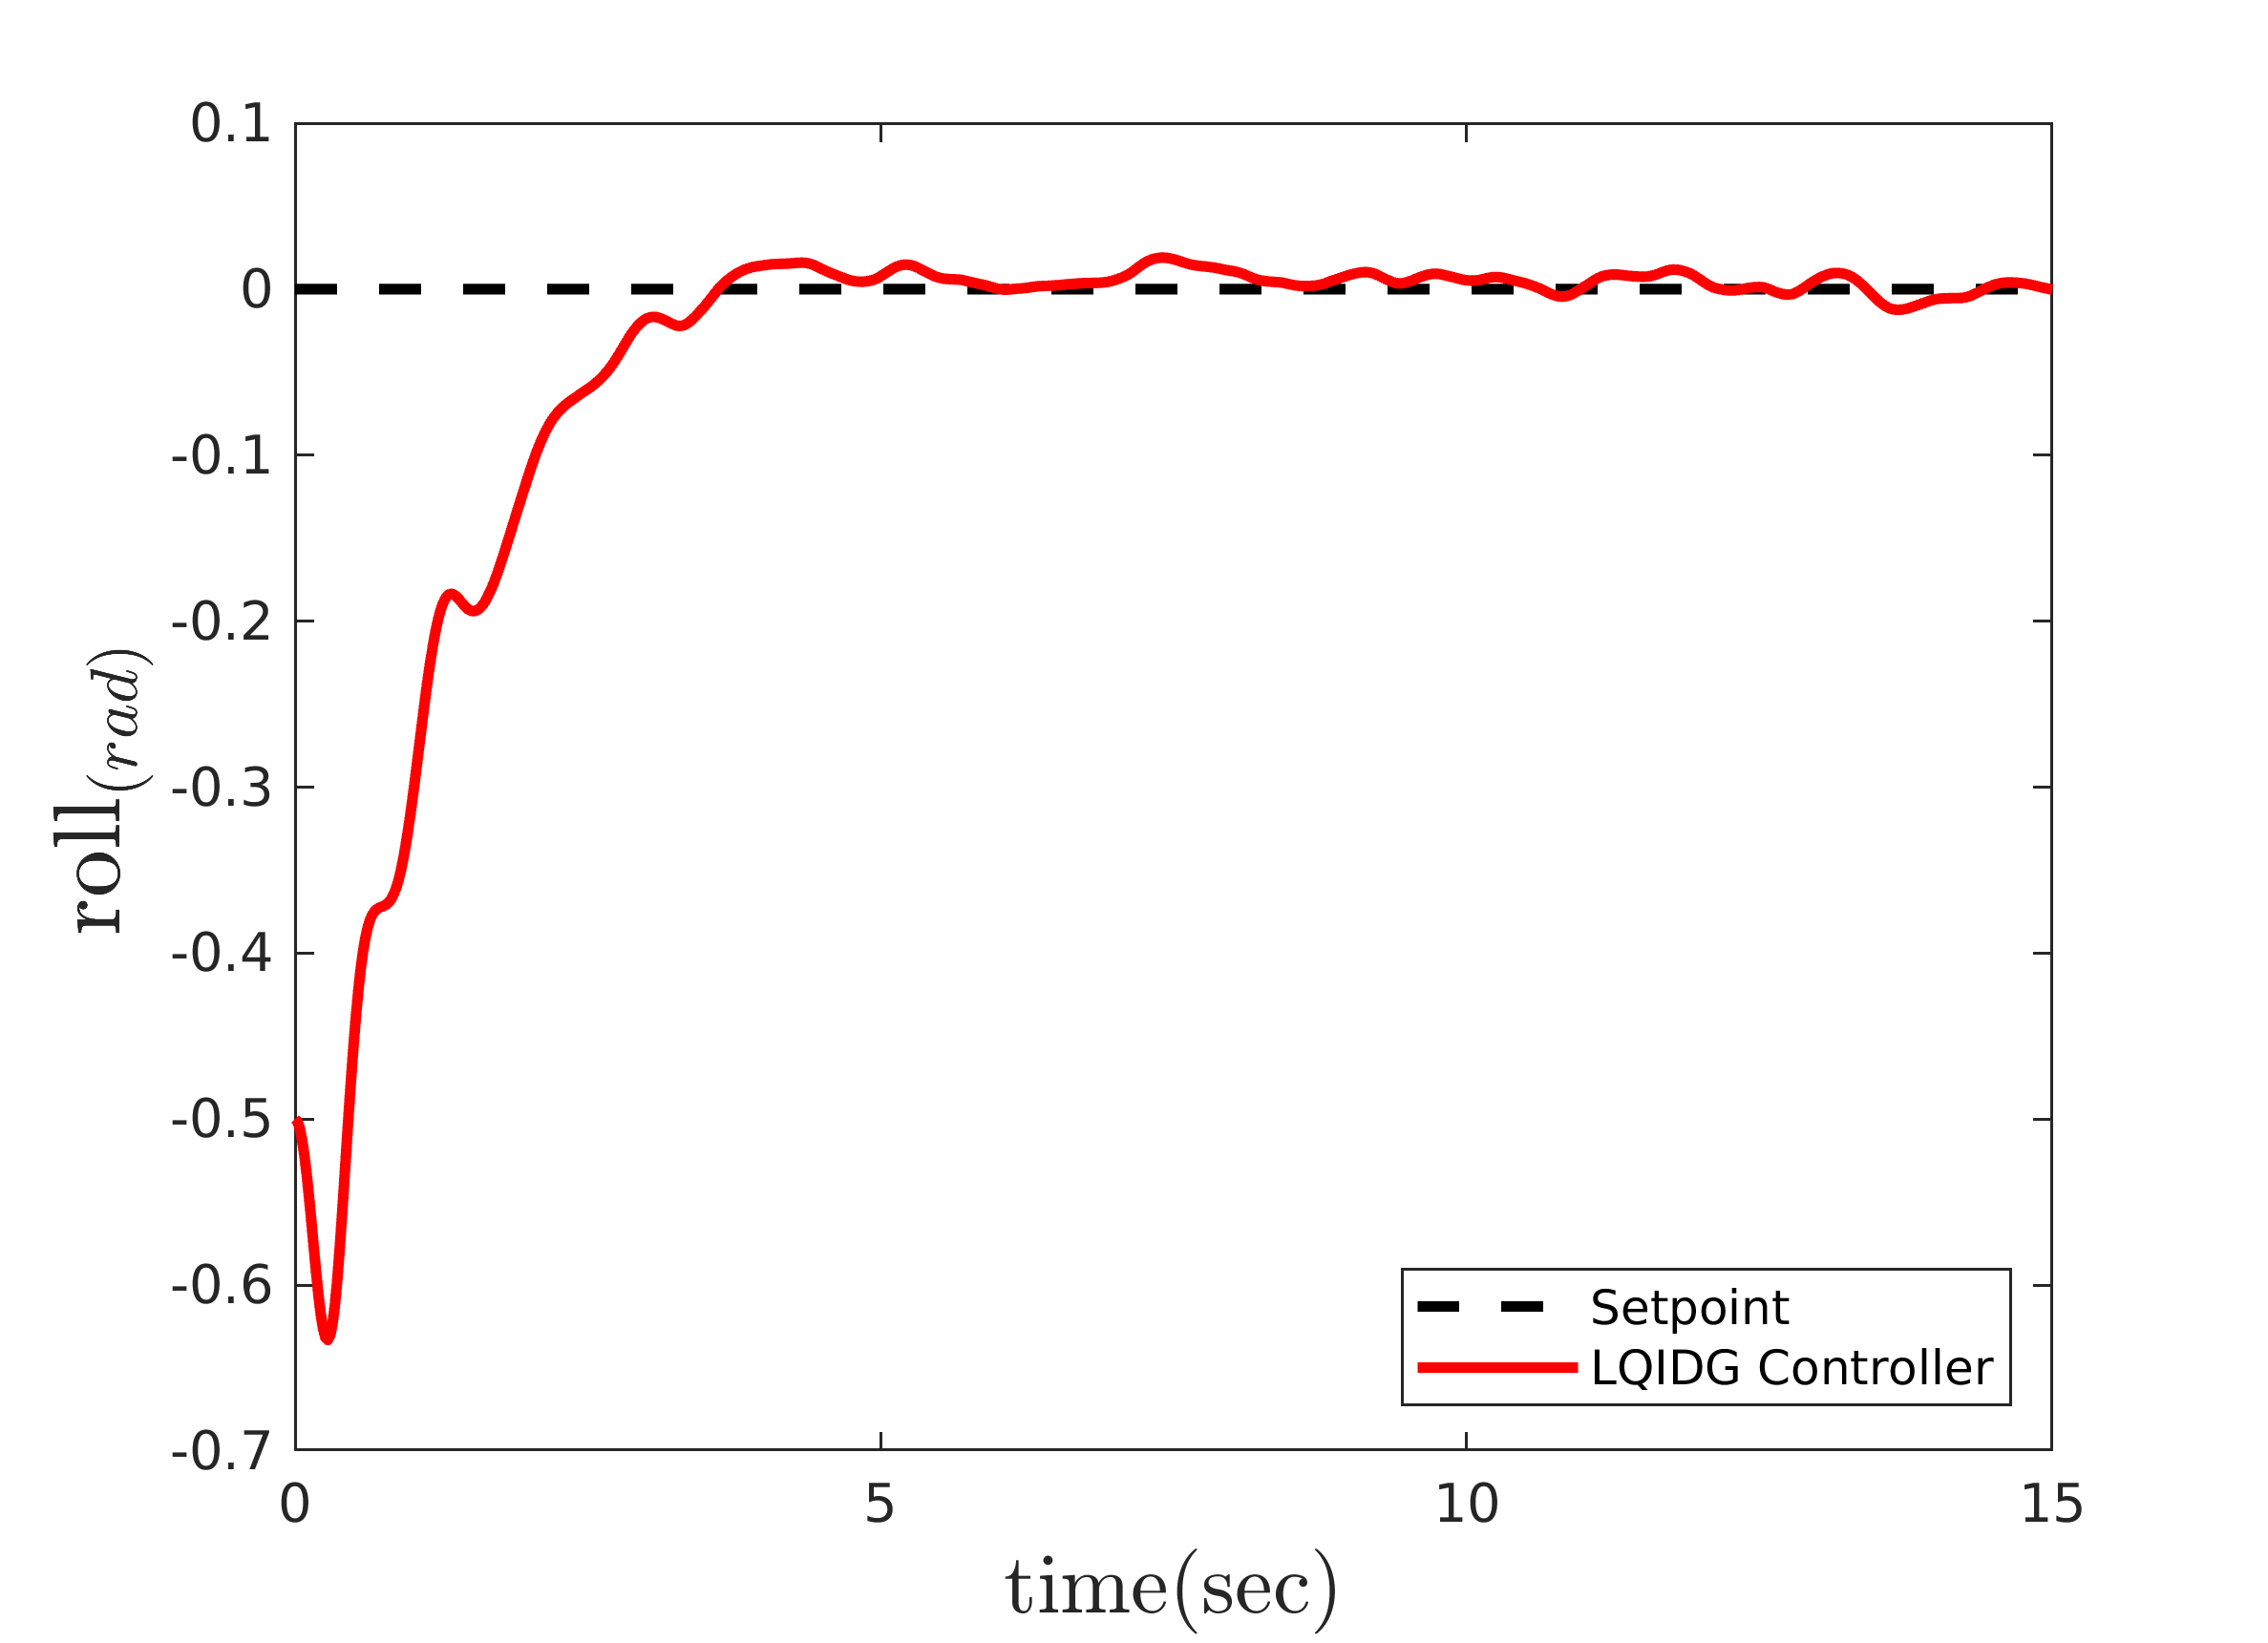
\includegraphics[width=12cm]{../Figures/MIL/LQIDG/3DOF/lqidg_roll.png}
%		\caption{تغییرات زاویه رول}
%	\end{subfigure}%
%	\begin{subfigure}
%		\centering
%		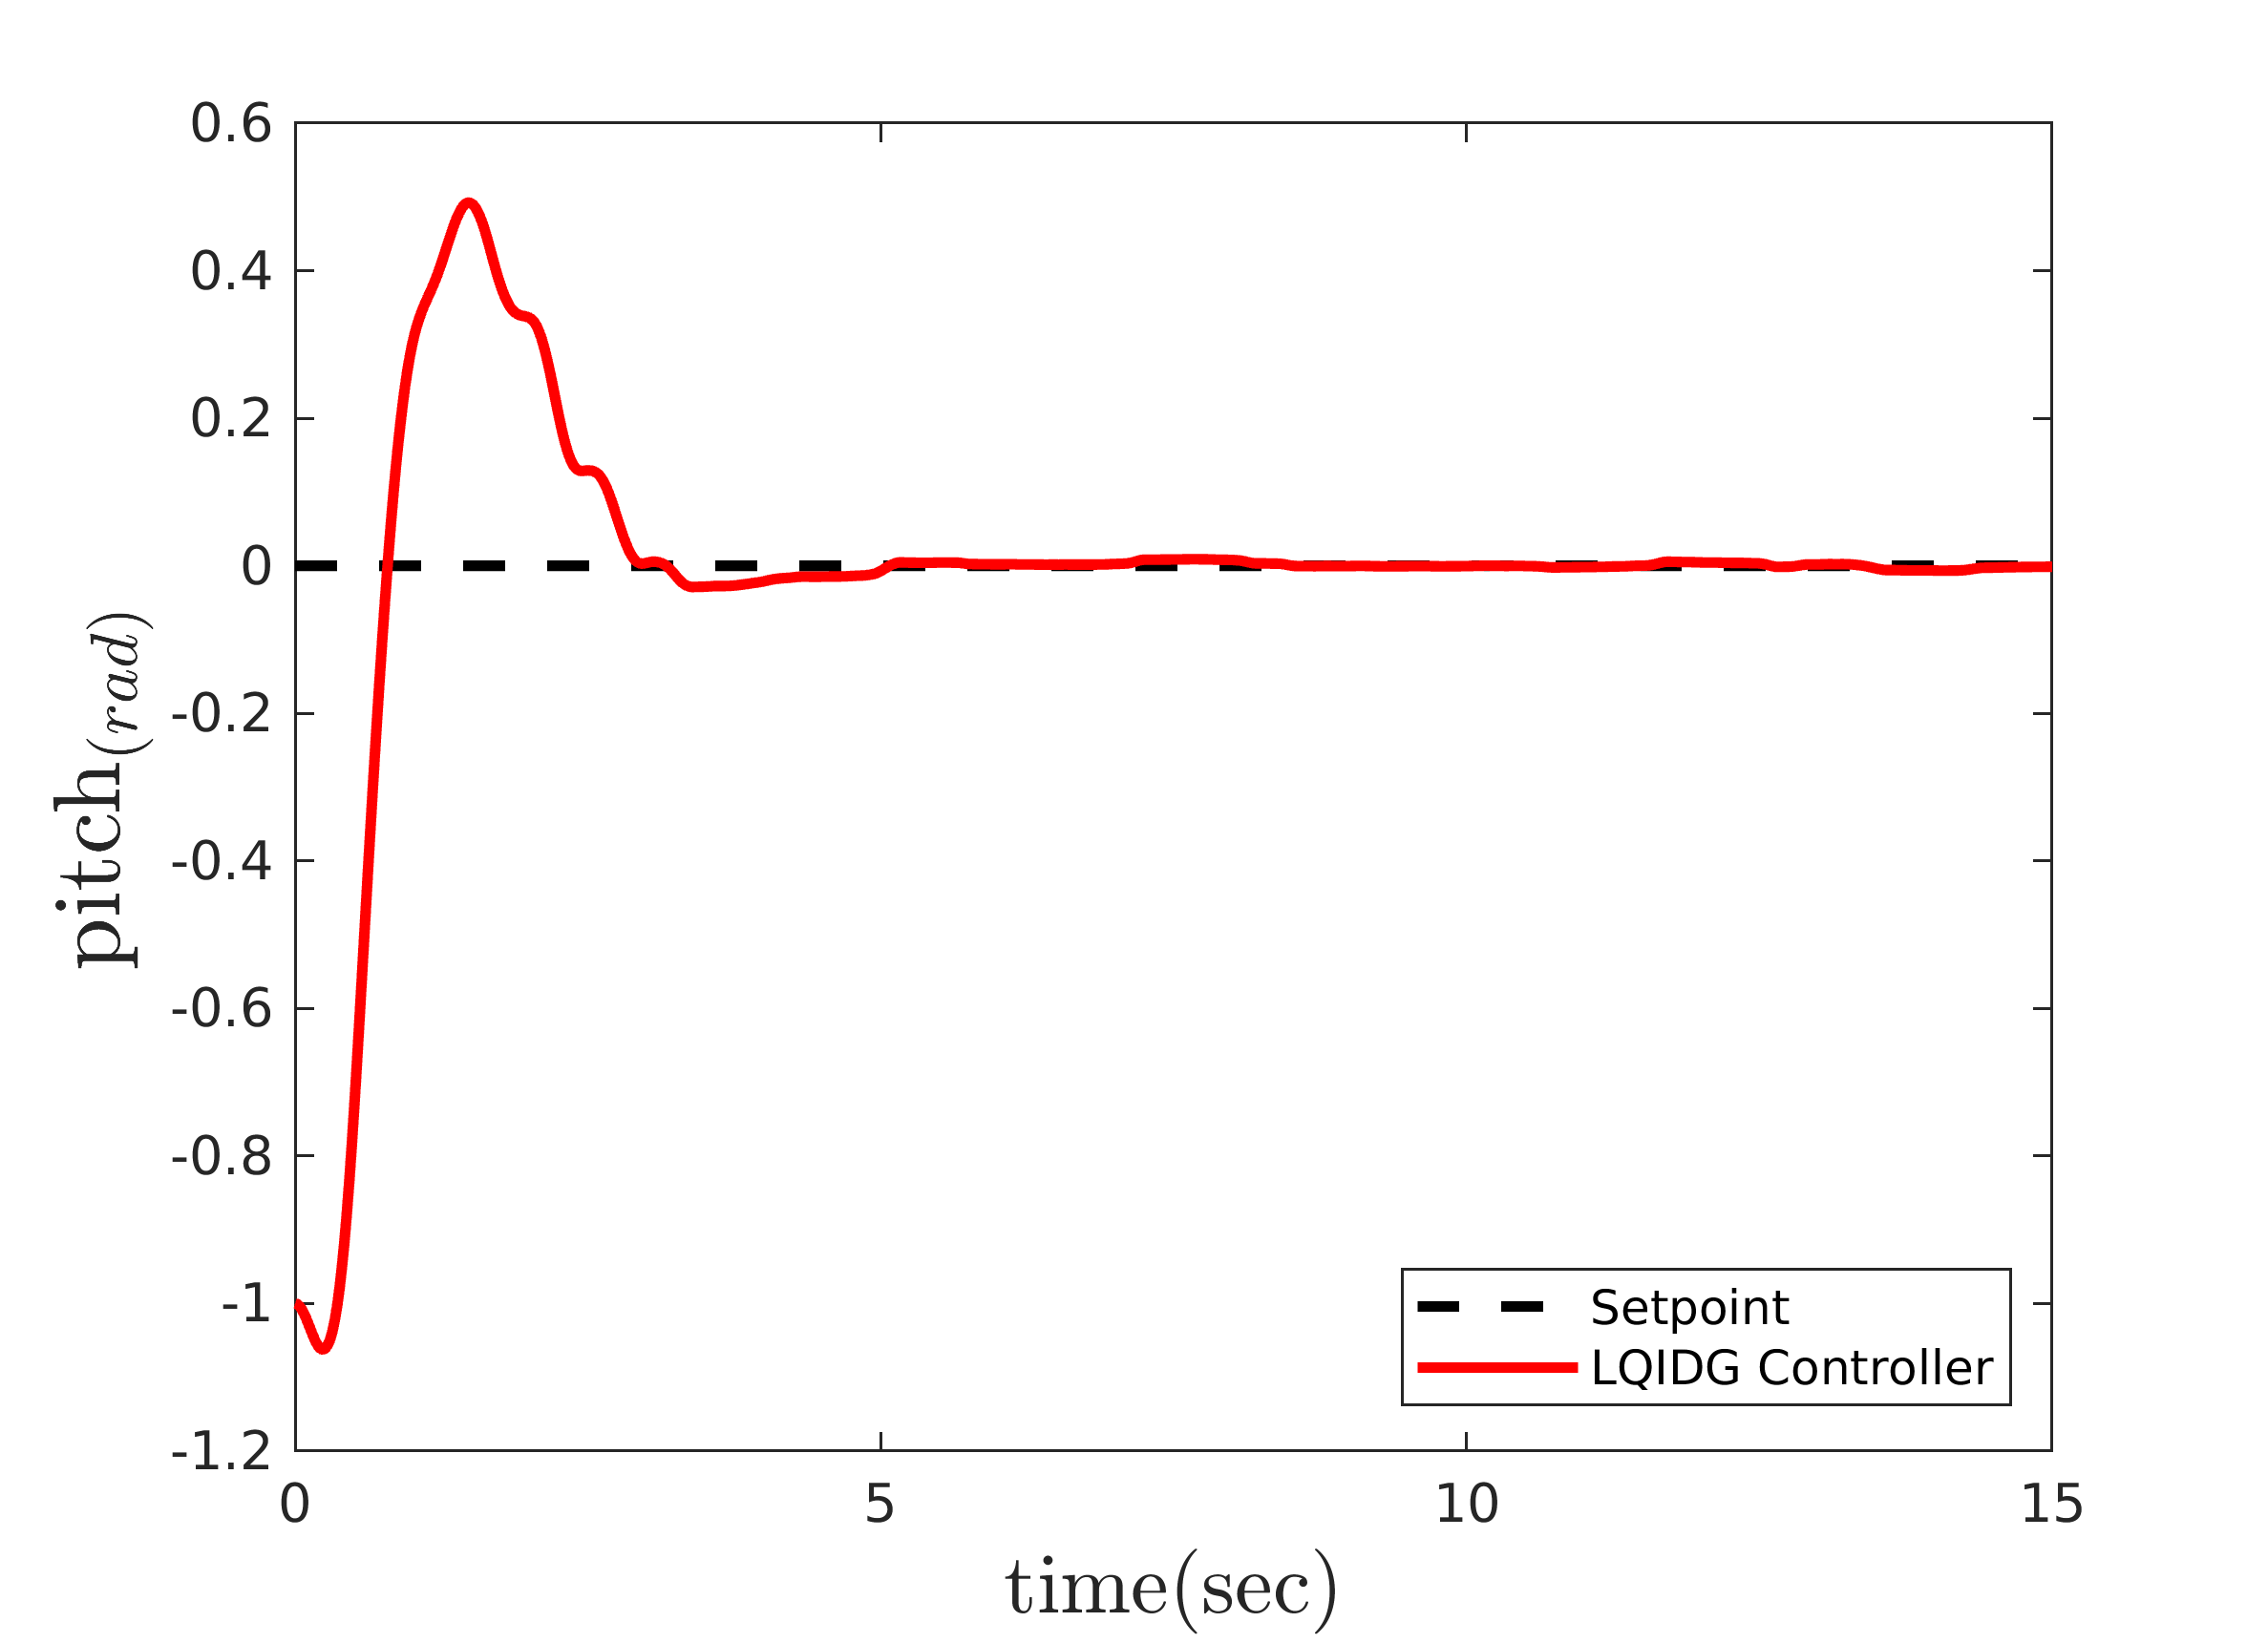
\includegraphics[width=12cm]{../Figures/MIL/LQIDG/3DOF/lqidg_pitch.png}
%		\caption{تغییرات زاویه پیچ}
%	\end{subfigure}
%	\caption{‫‪عملکرد کنترل‌کننده LQIDG در کنترل زاویه رول، پیچ و یاد (تعقیب ورودی صفر)}
%\end{figure}
%
%\begin{figure}[H]
%	\centering
%	\begin{subfigure}[H]
%		\centering
%		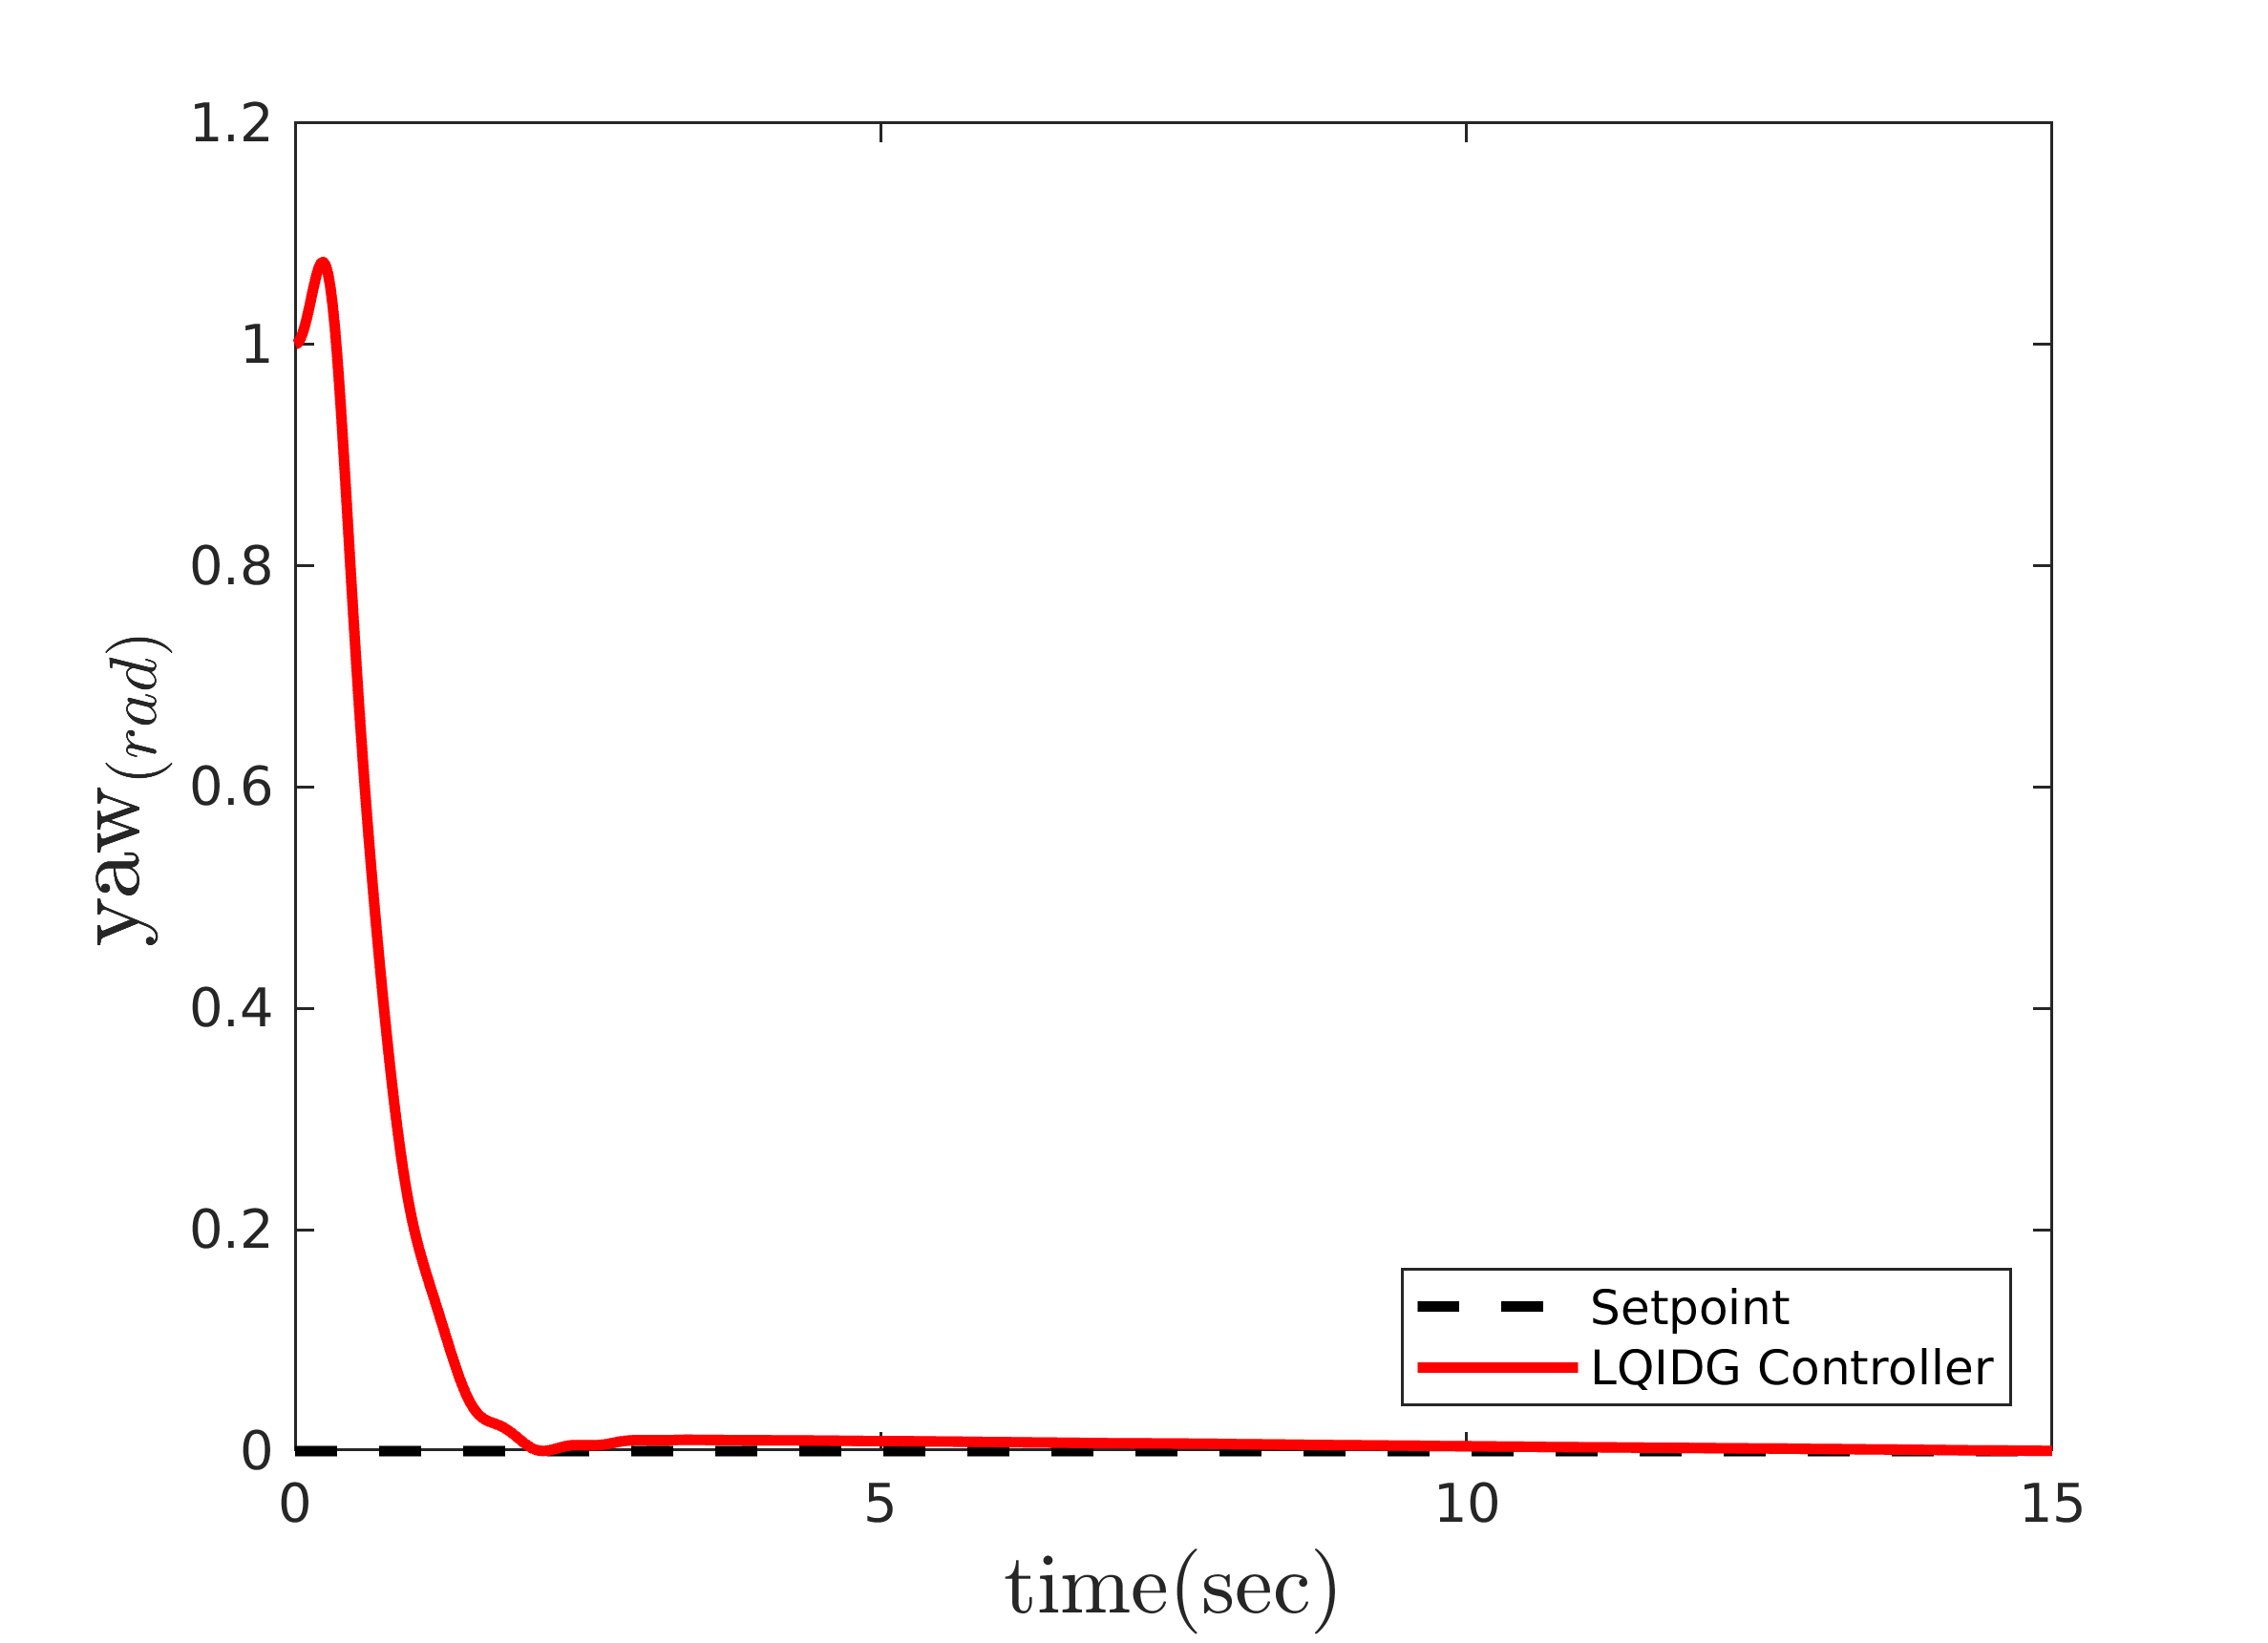
\includegraphics[width=12cm]{../Figures/MIL/LQIDG/3DOF/lqidg_yaw.png}
%		\caption{تغییرات زاویه یاو}
%	\end{subfigure}
%	\caption{‫‪عملکرد کنترل‌کننده LQIDG در کنترل زاویه رول، پیچ و یاد (تعقیب ورودی صفر)}
%\end{figure}
\begin{figure}[H]
	\centering
\subfigure[تغییرات زاویه رول]{
	\centering
	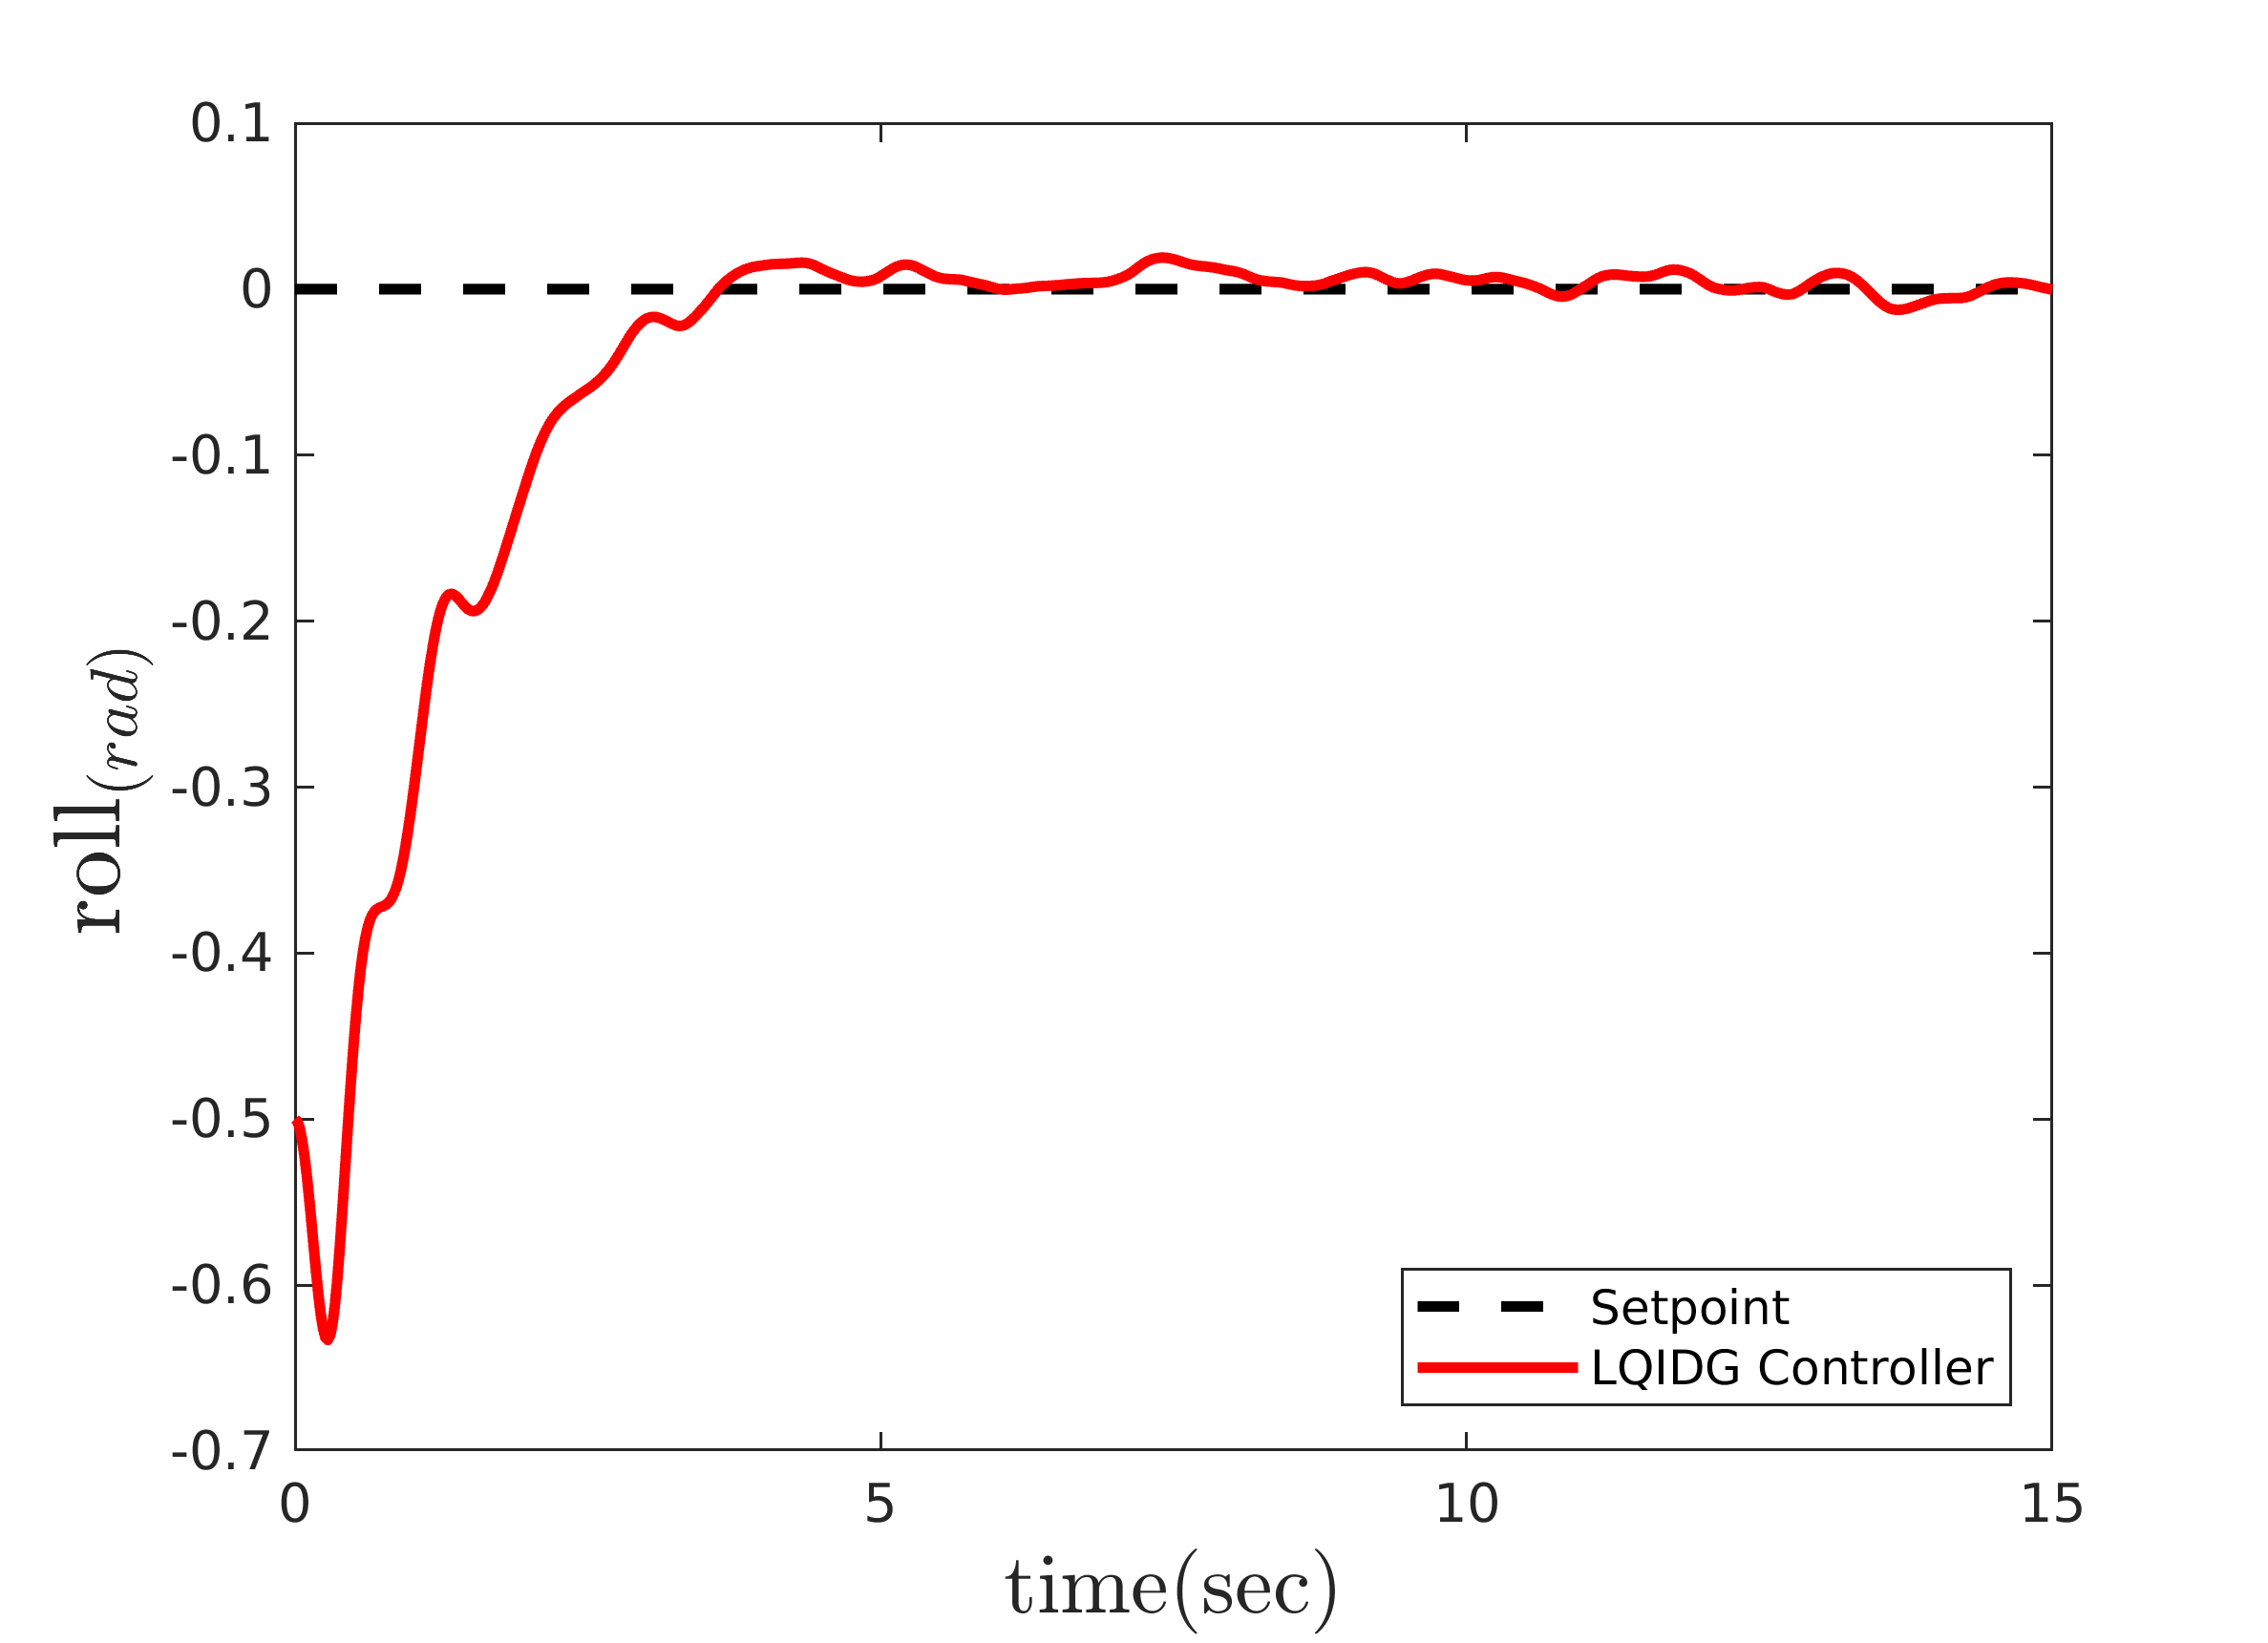
\includegraphics[width=.48\linewidth]{../Figures/MIL/LQIDG/3DOF/lqidg_roll.png}
}
\subfigure[تغییرات زاویه پیچ]{
	\centering
	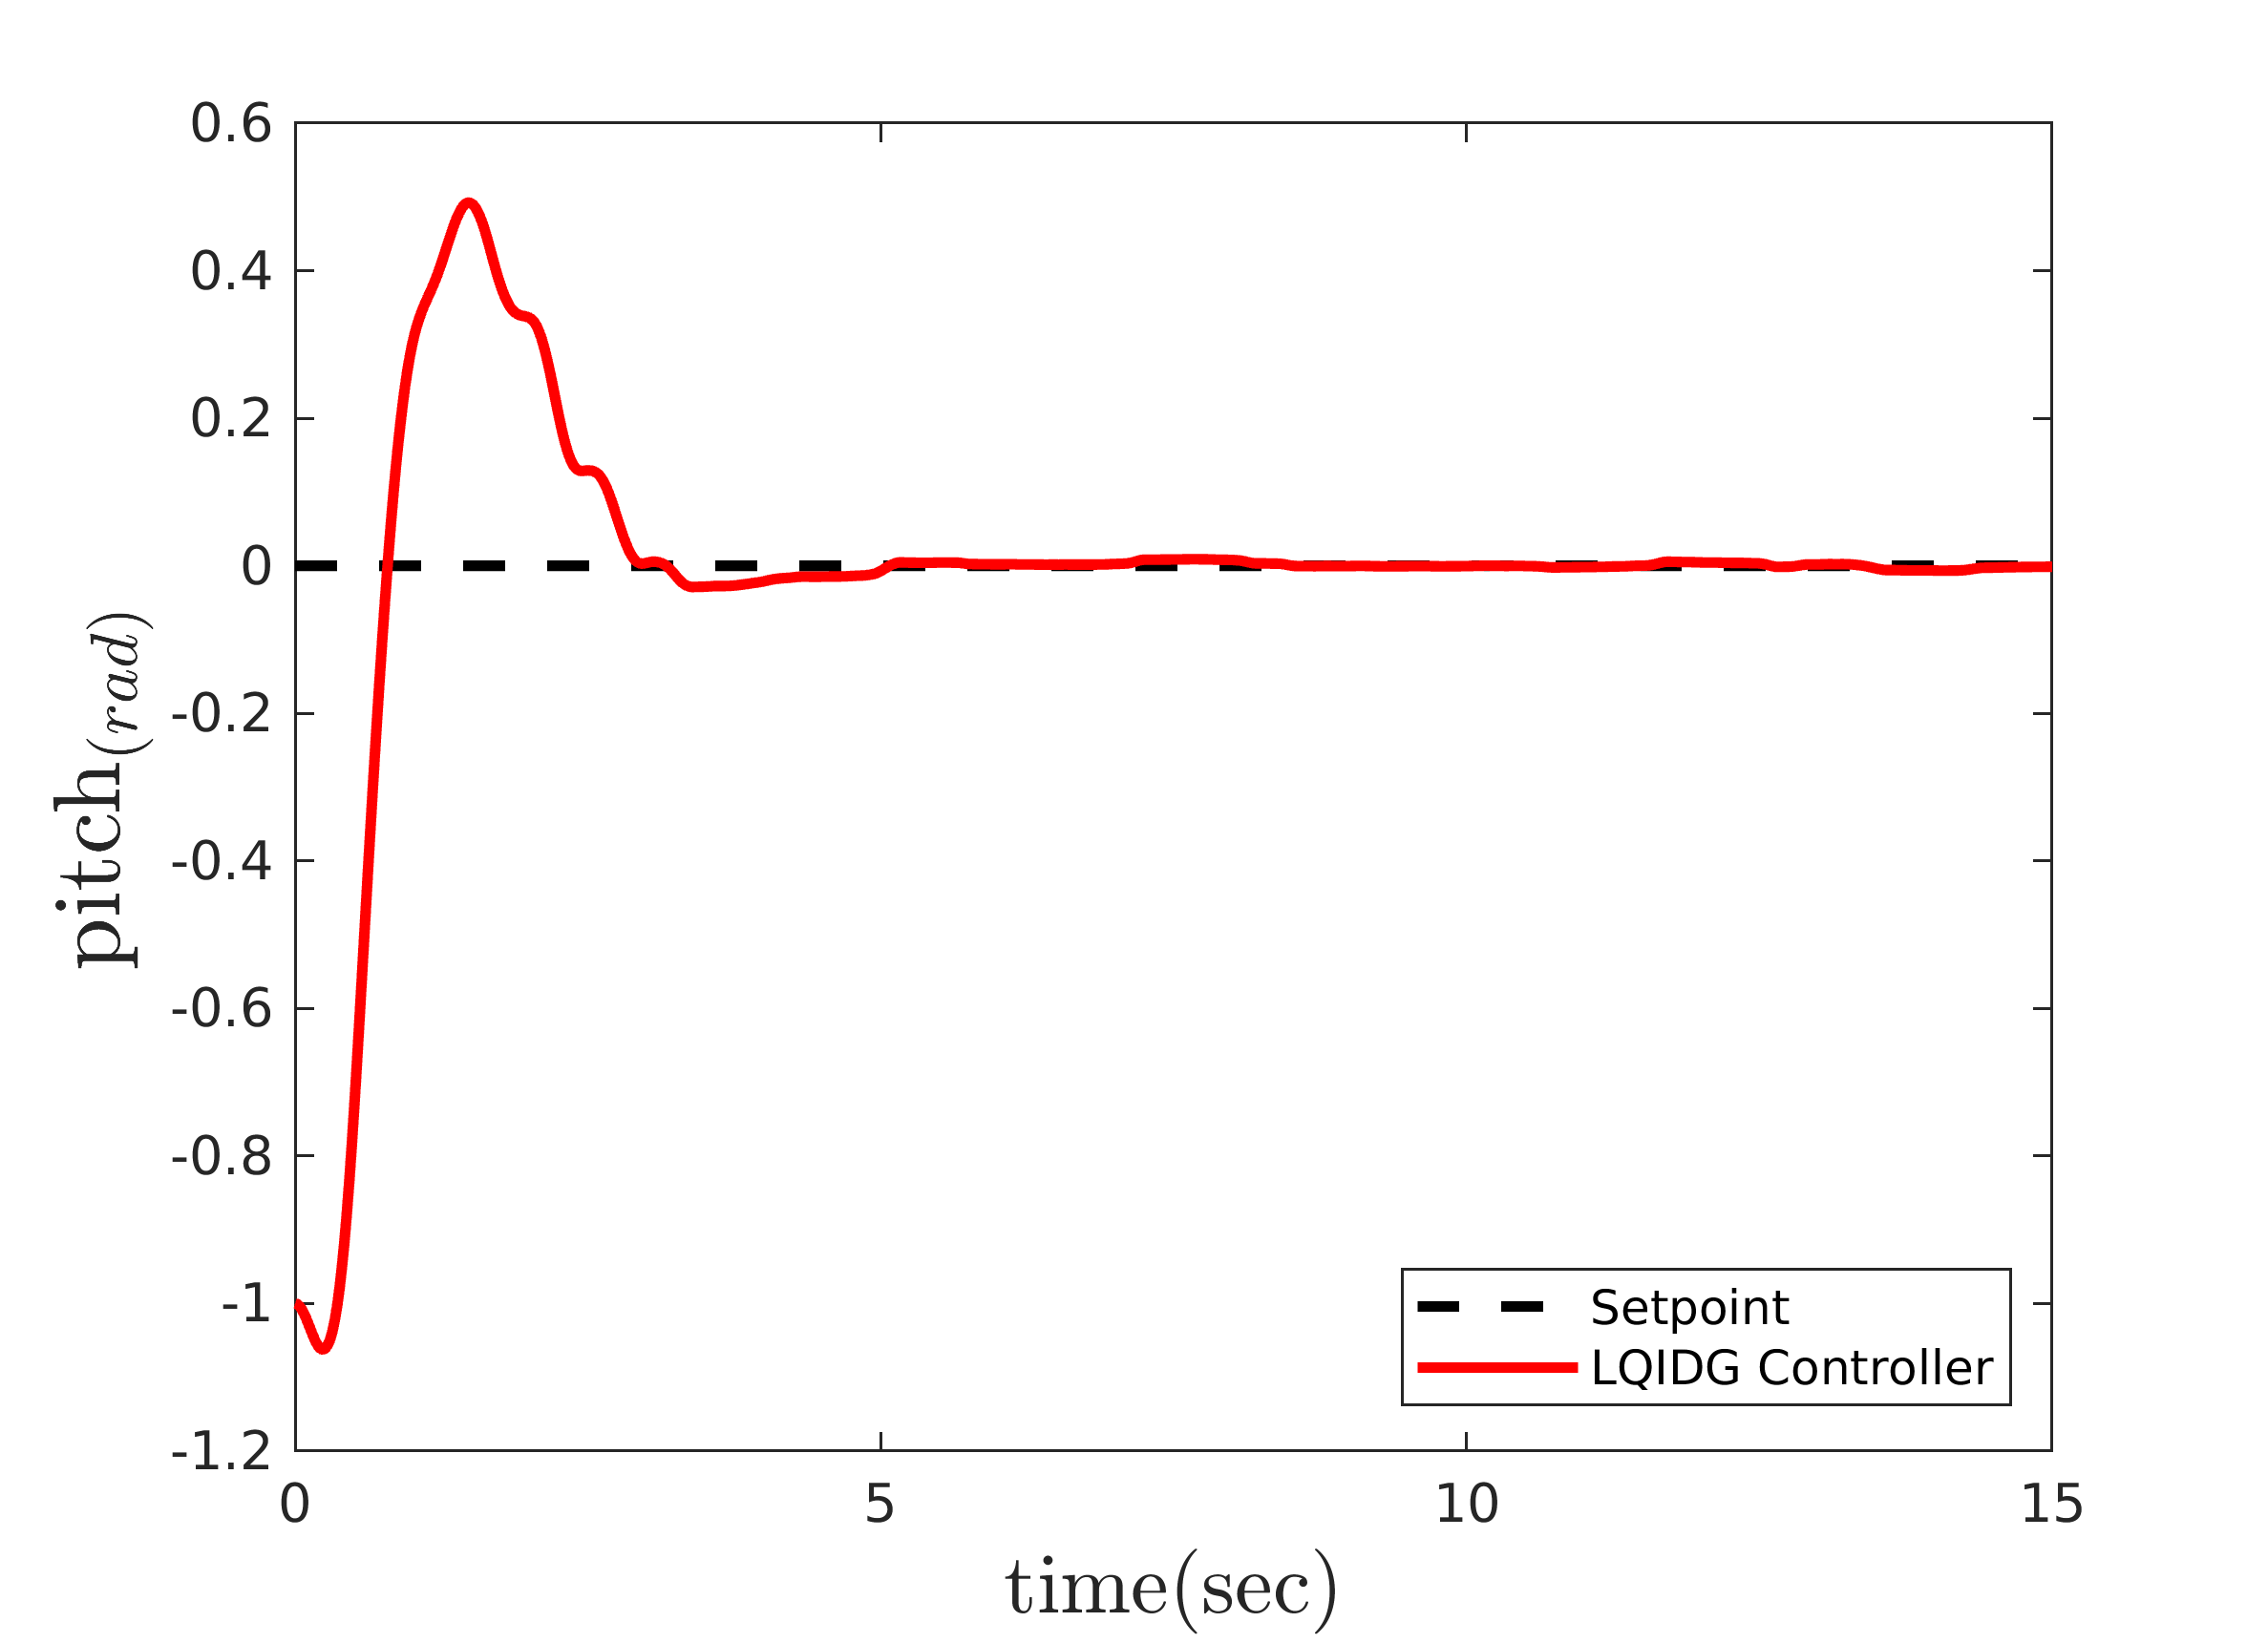
\includegraphics[width=.48\linewidth]{../Figures/MIL/LQIDG/3DOF/lqidg_pitch.png}
}
\subfigure[تغییرات زاویه یاو]{
	\centering
	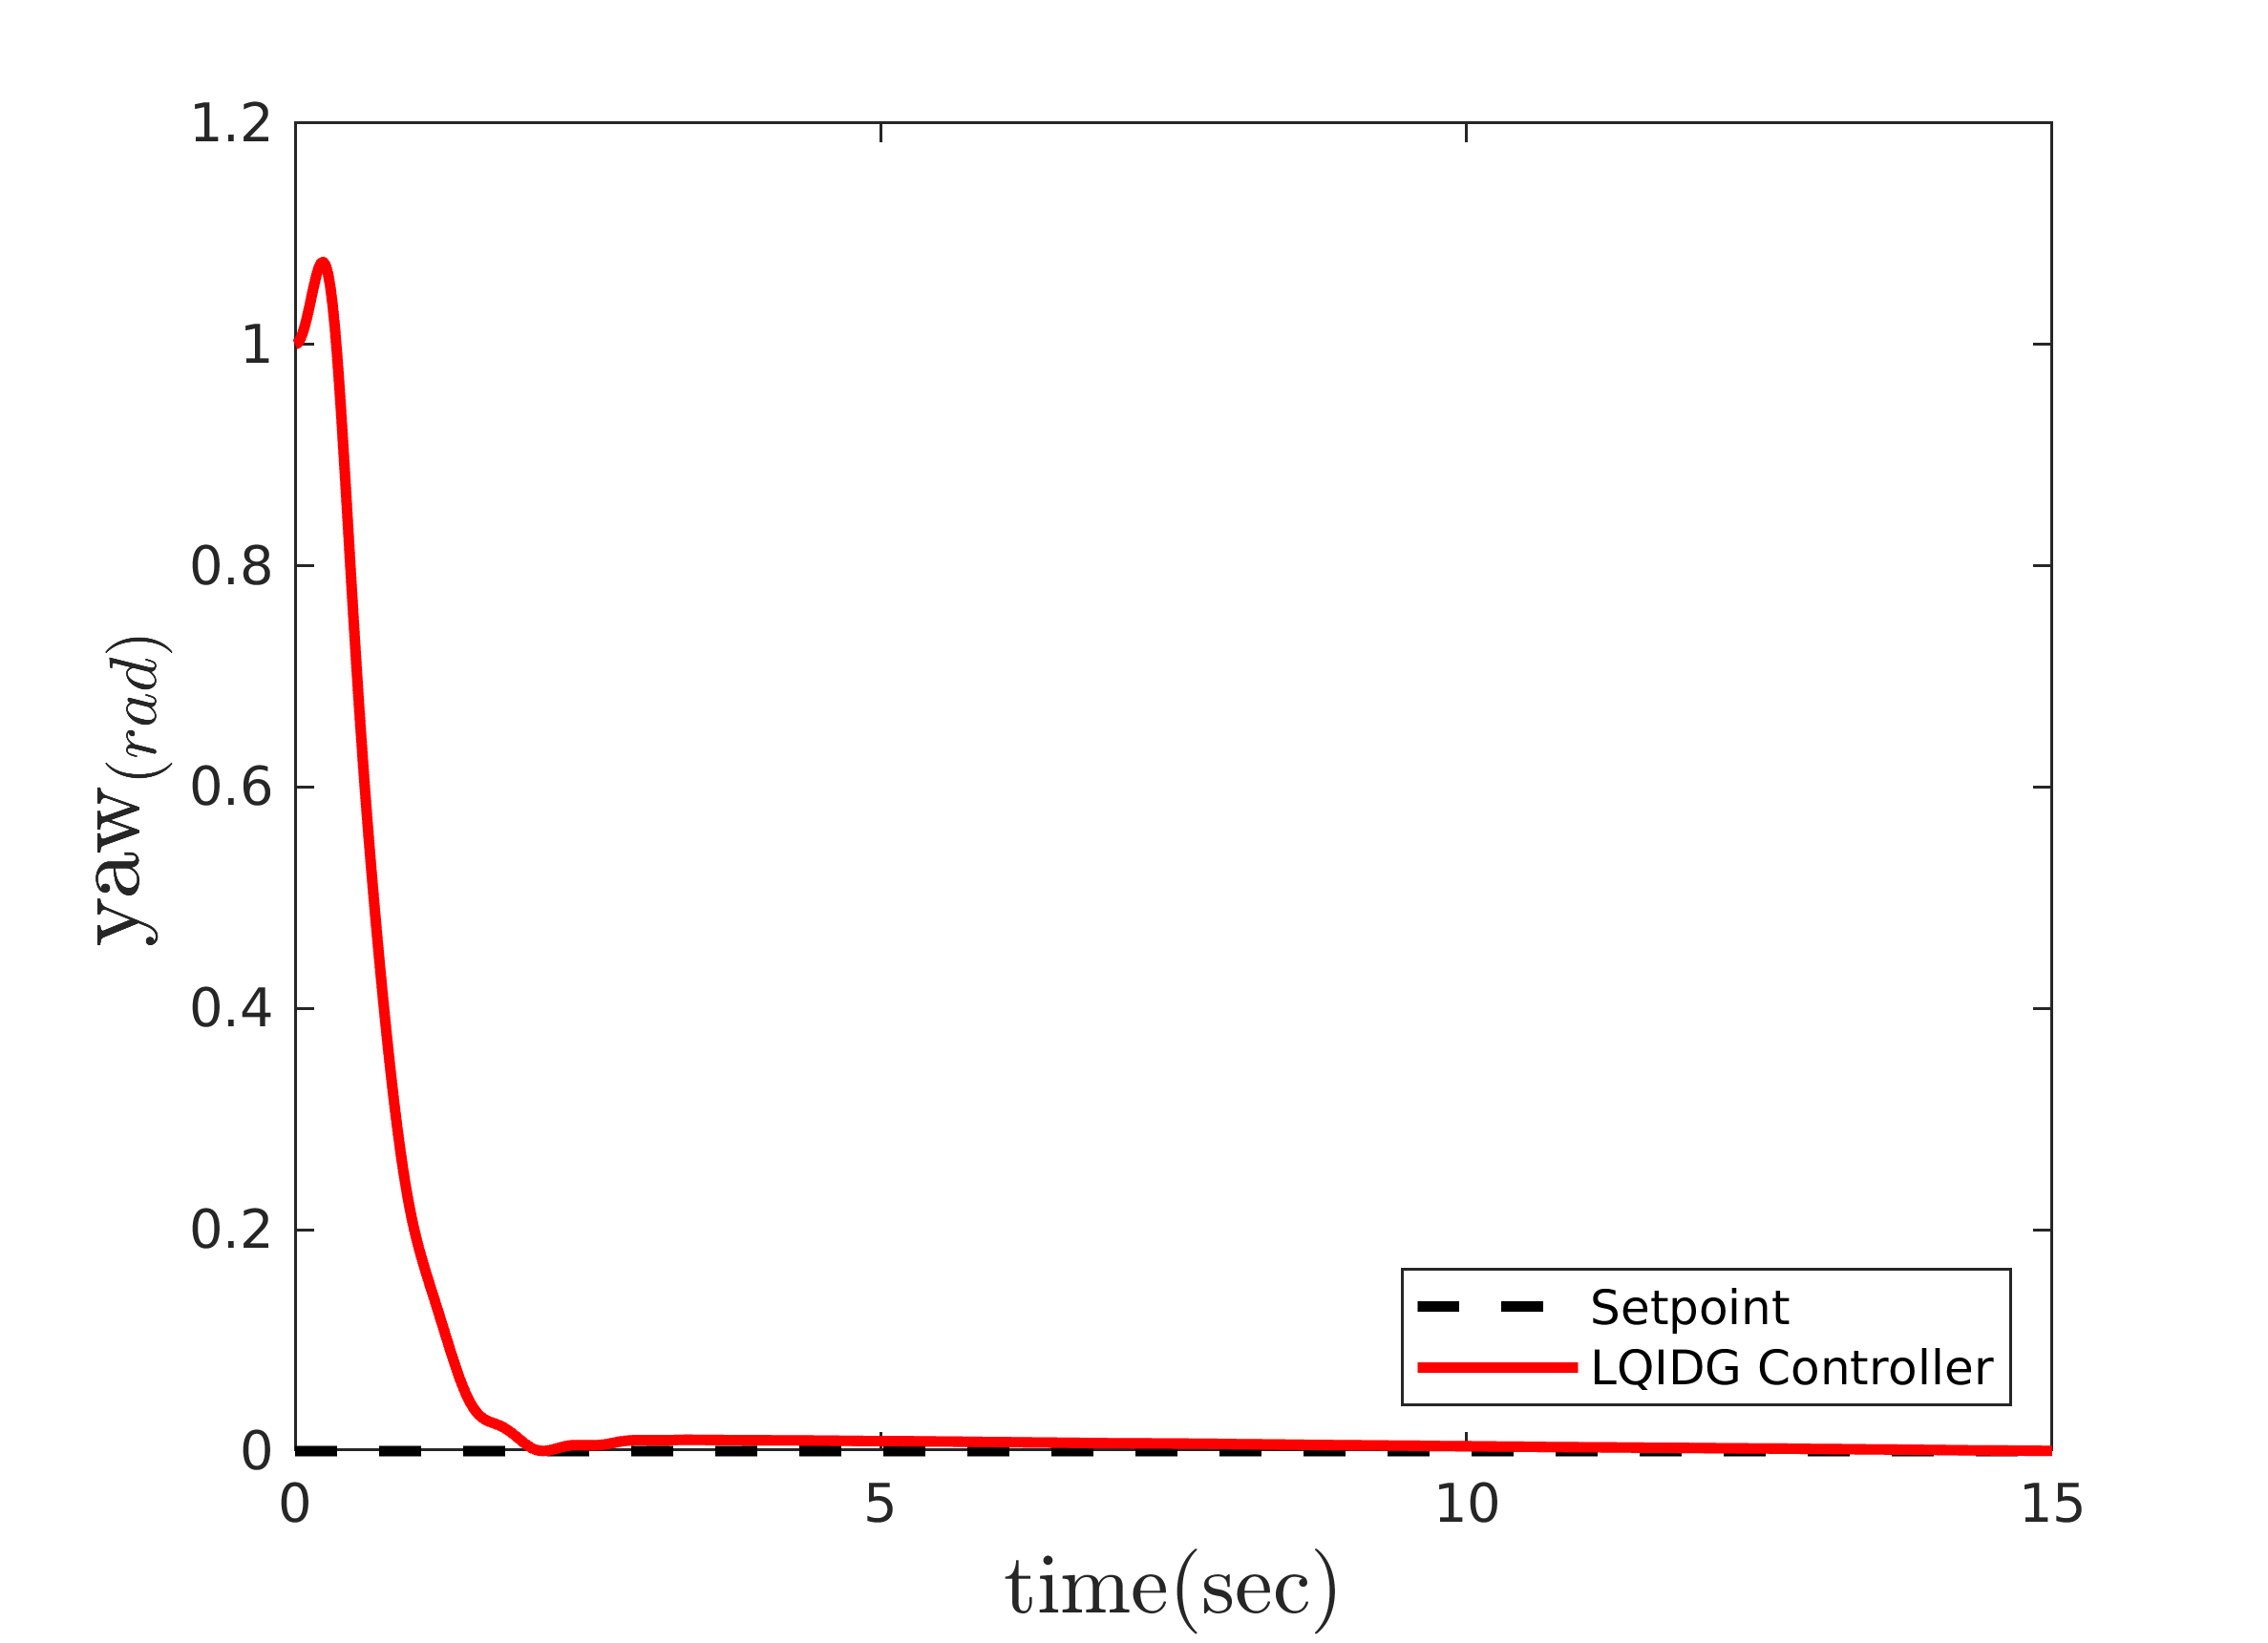
\includegraphics[width=.48\linewidth]{../Figures/MIL/LQIDG/3DOF/lqidg_yaw.png}
}
	\caption{‫‪عملکرد کنترل‌کننده \lr{LQIDG} در کنترل وضعیت با حضور نويز اندازه‌گیری}
	\label{lqidg_roll_pitch_yaw_fig_simulation}
\end{figure}


\begin{figure}[H]
	\centering
	\subfigure[موتور شماره یک]{
		\centering
		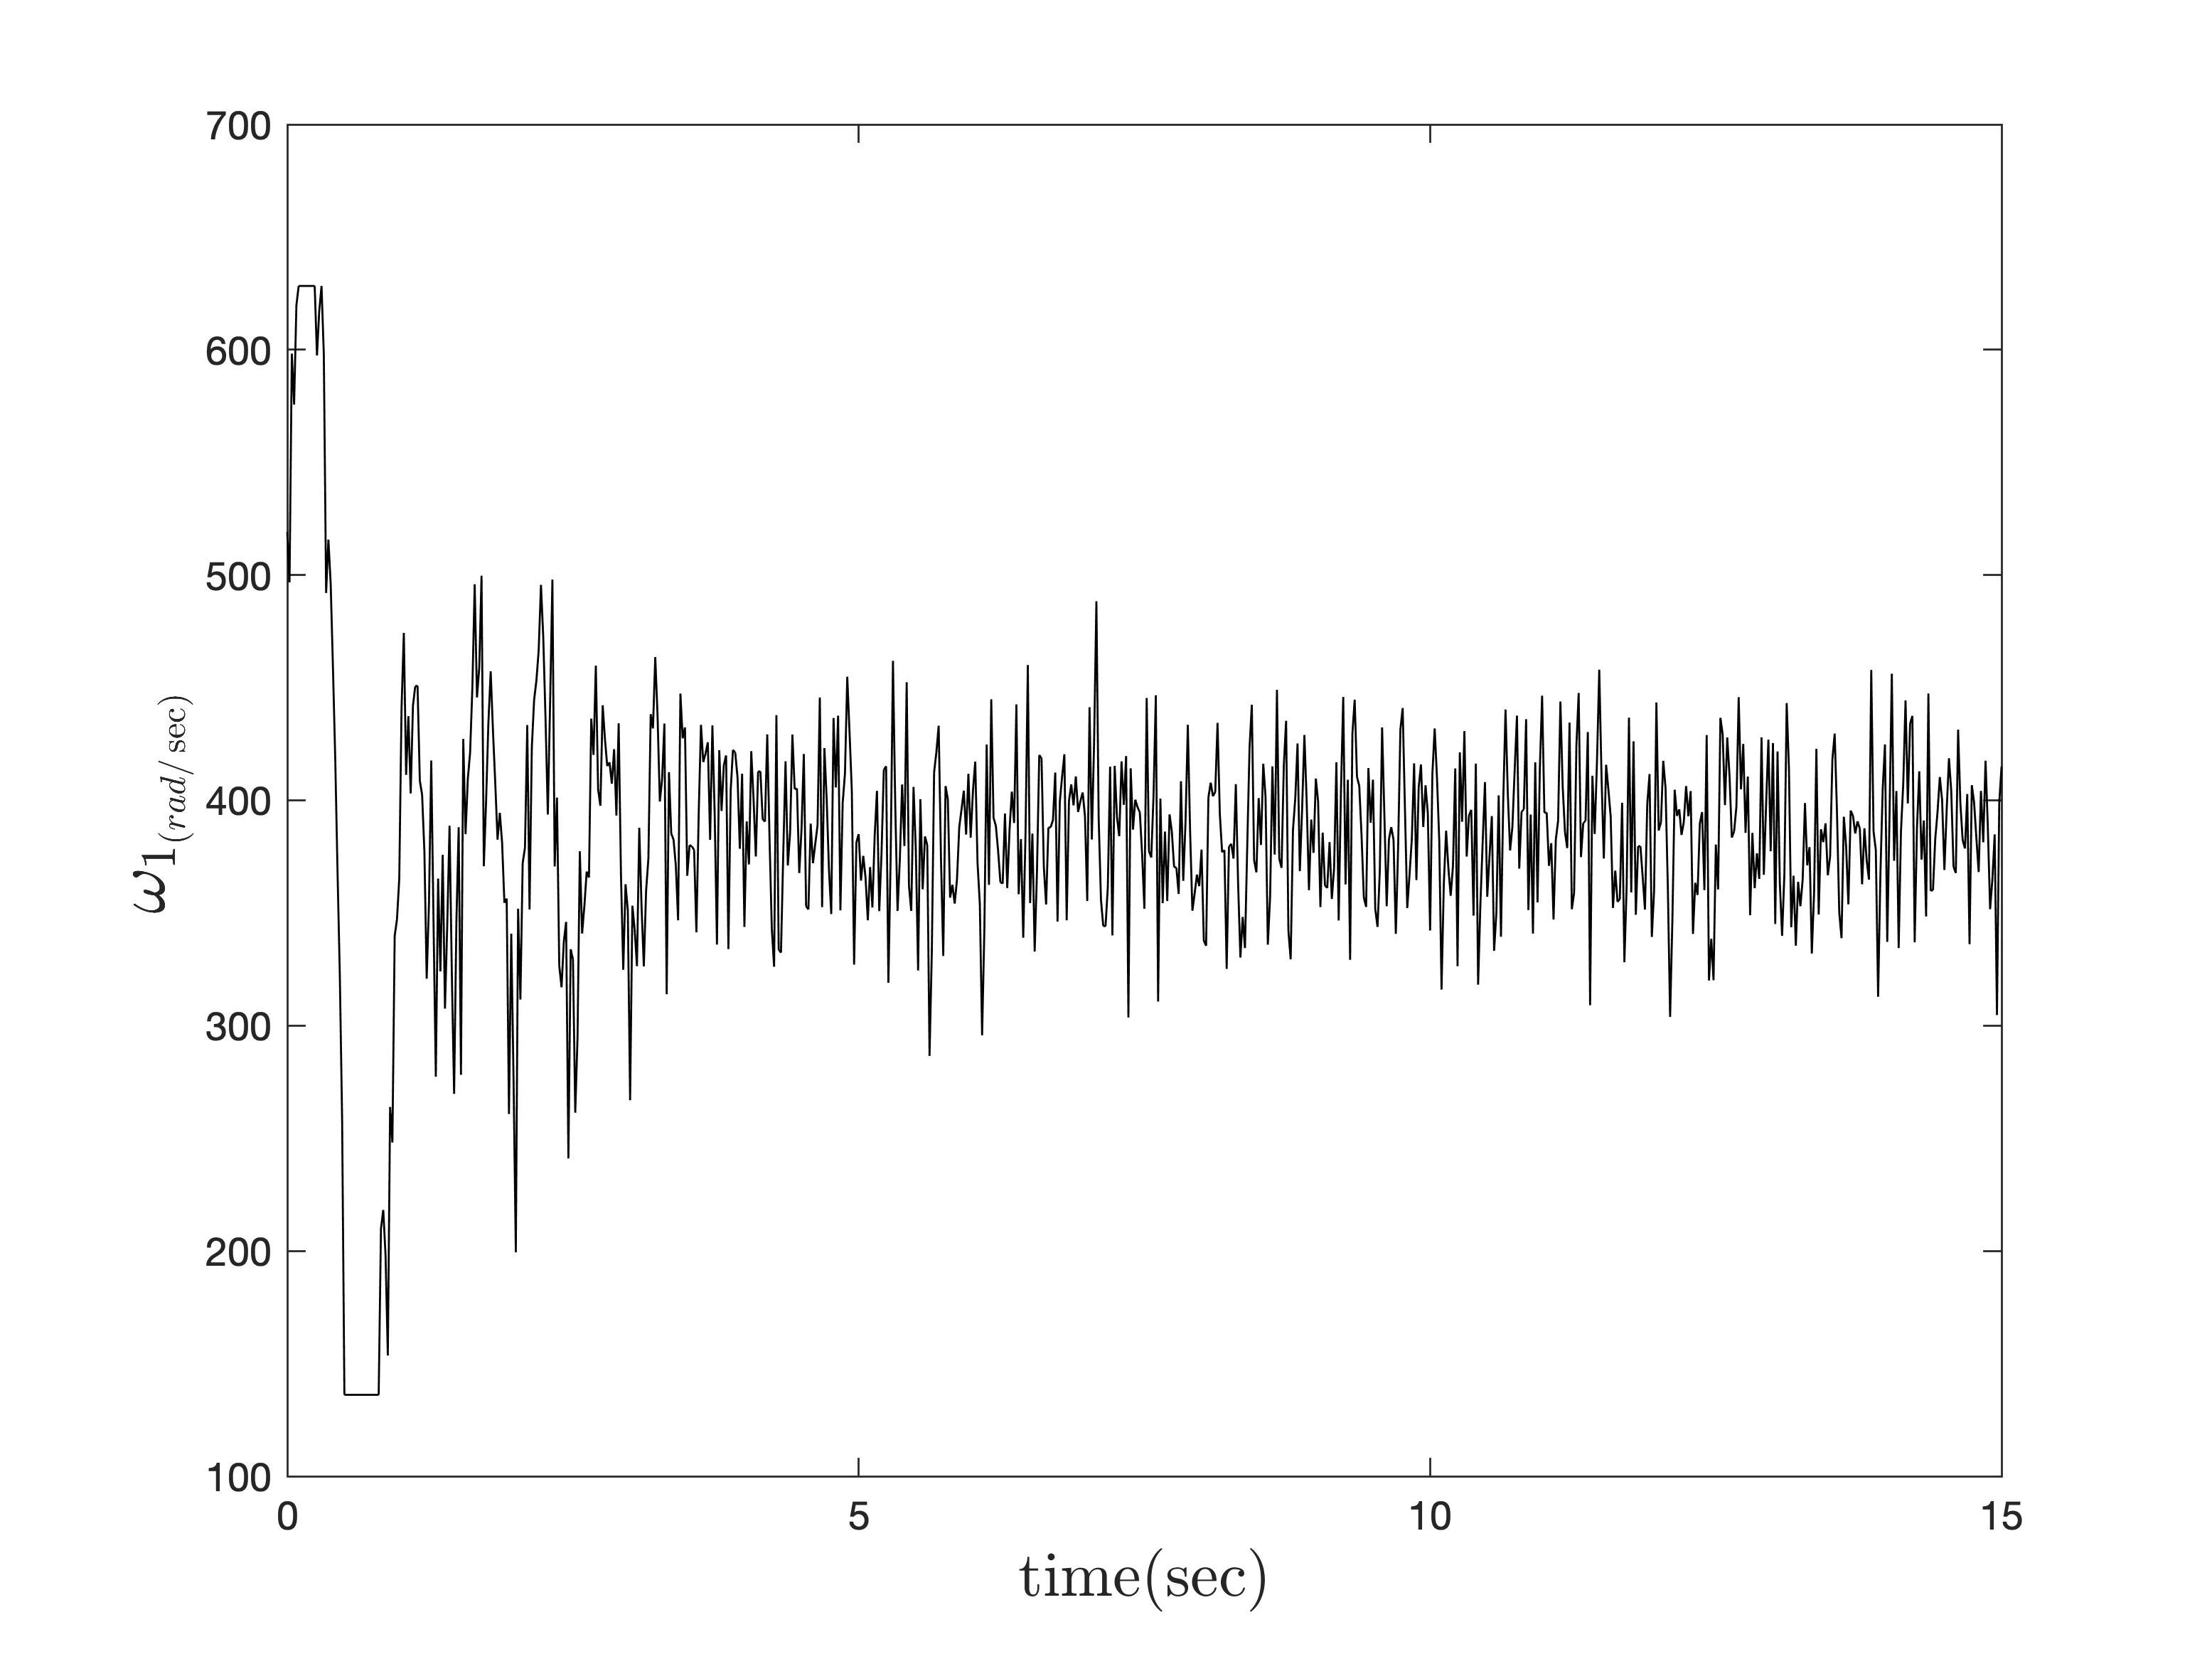
\includegraphics[width=.45\linewidth]{../Figures/MIL/LQIDG/3DOF/lqidg_roll_pitch_Omega_1.png}
	}
	\subfigure[موتور شماره دو]{
		\centering
		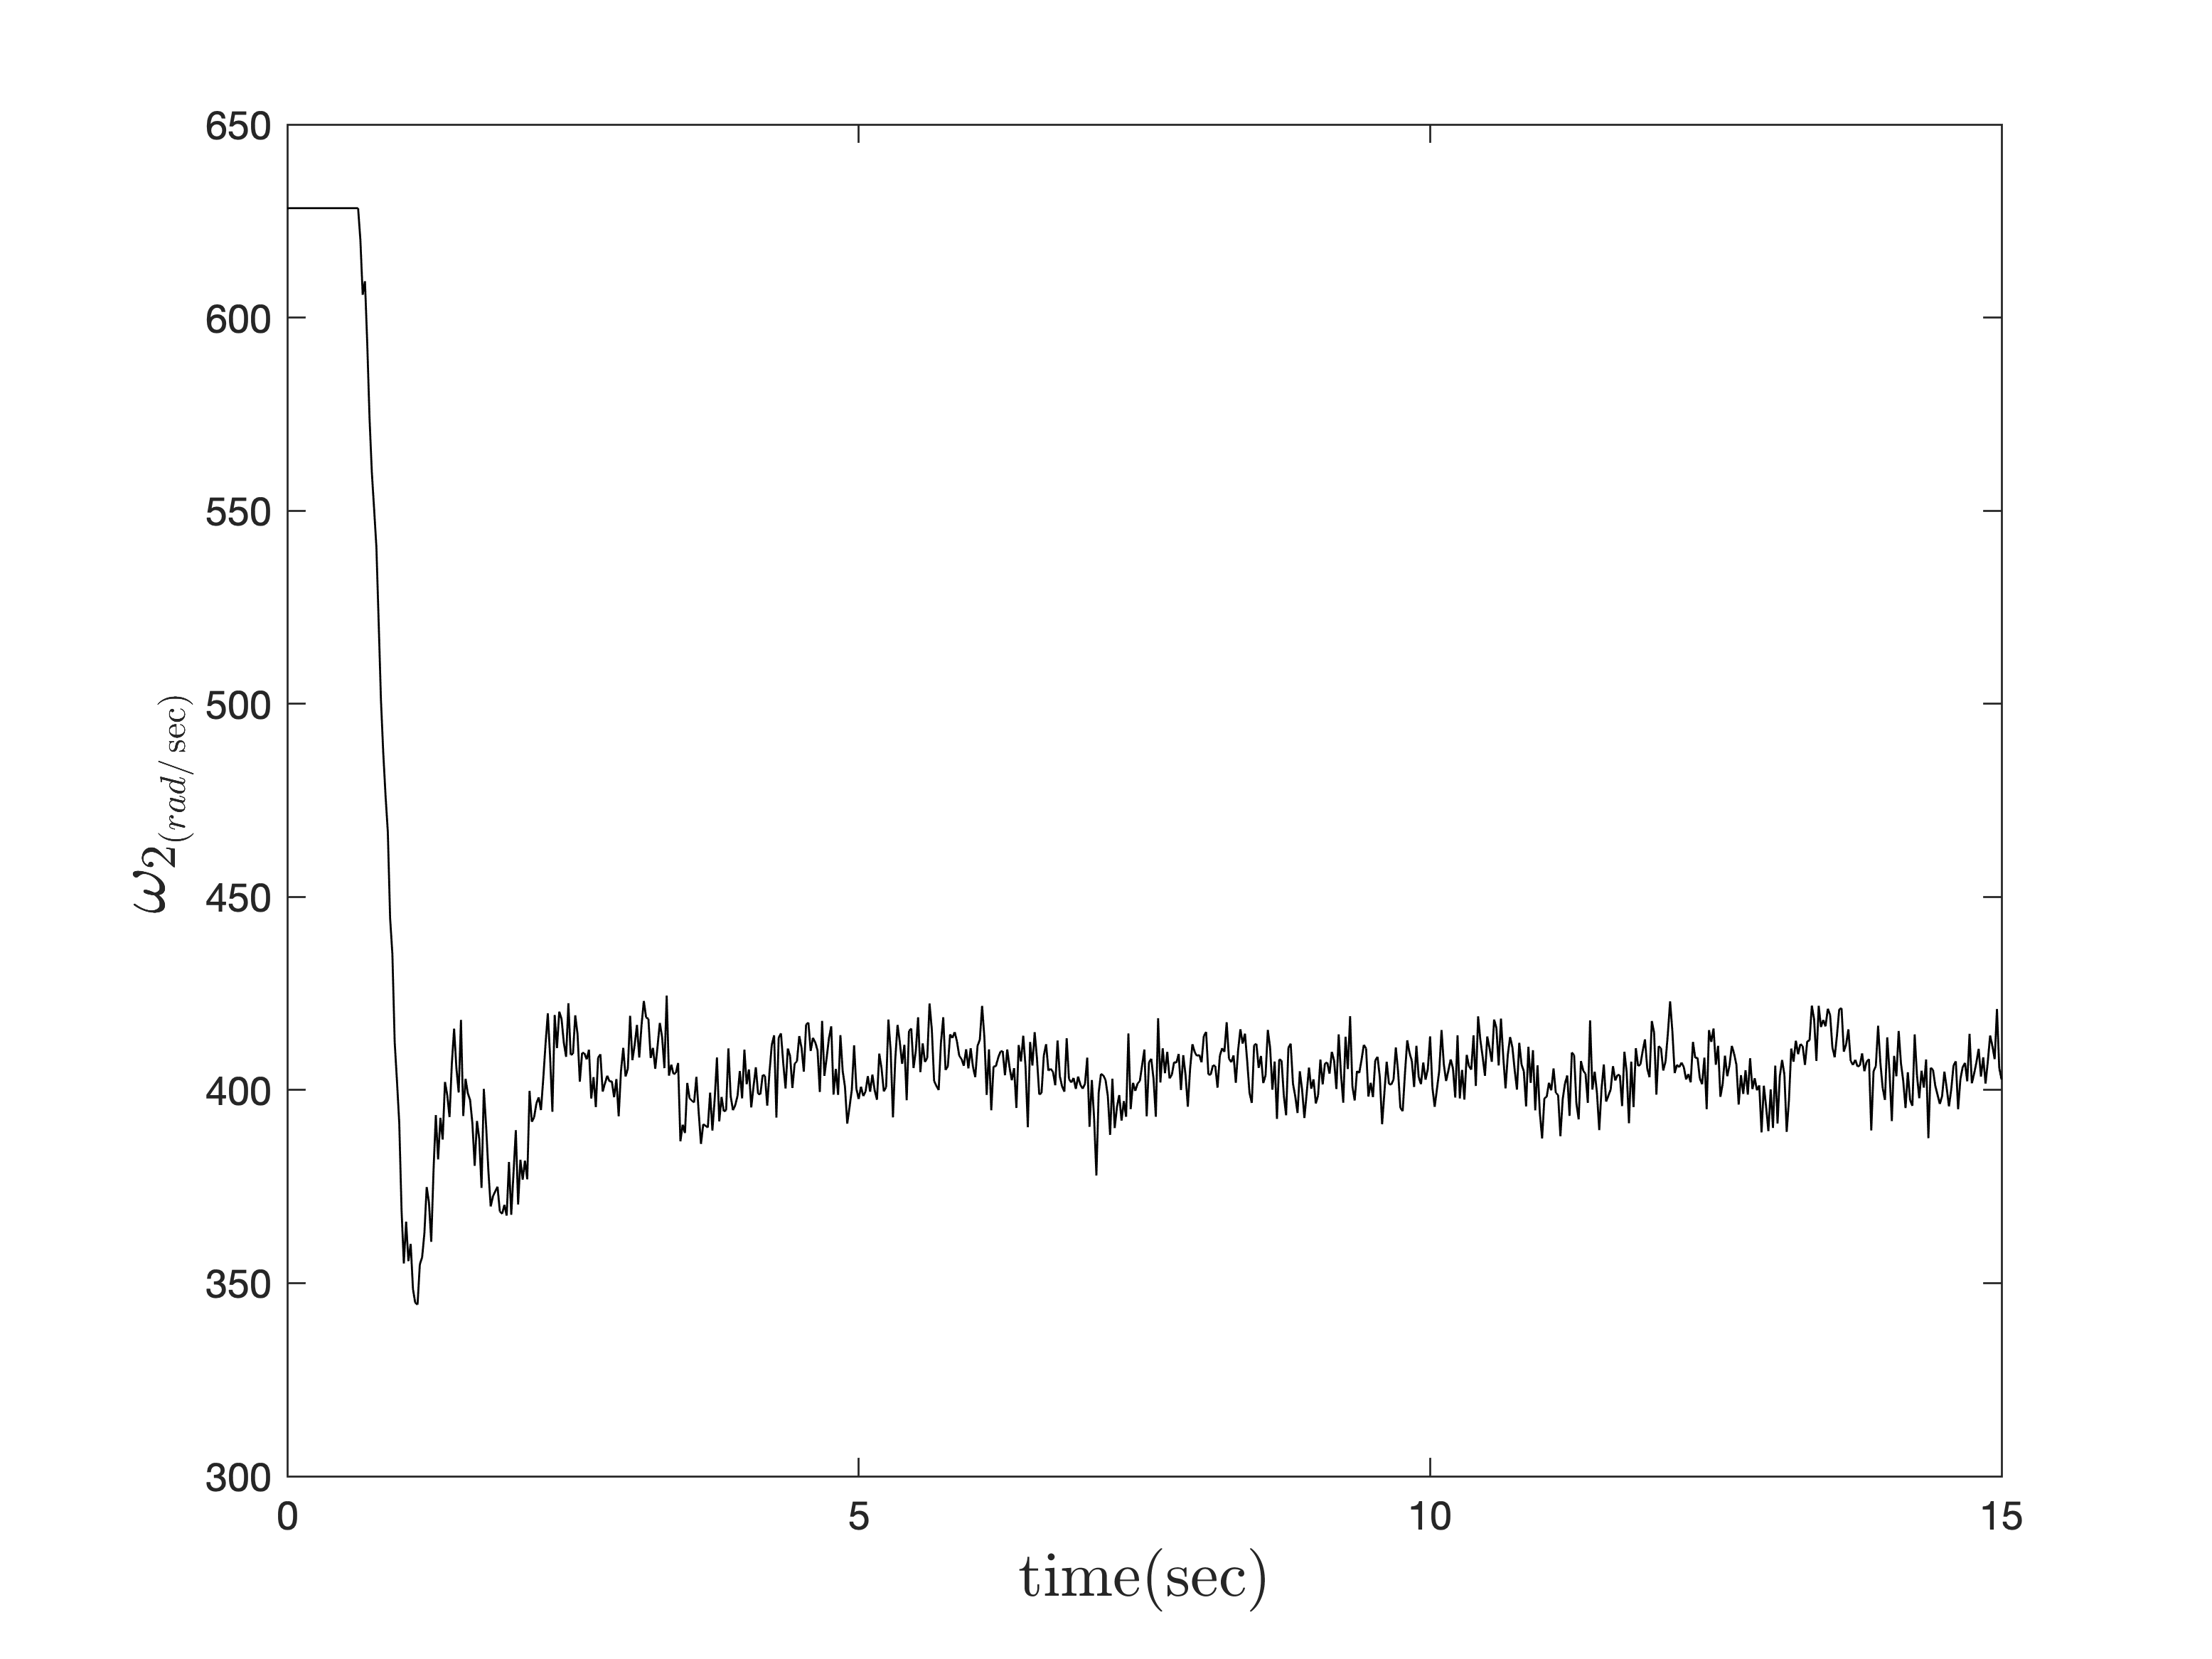
\includegraphics[width=.45\linewidth]{../Figures/MIL/LQIDG/3DOF/lqidg_roll_pitch_Omega_2.png}
	}
	\subfigure[موتور شماره سه]{
		\centering
		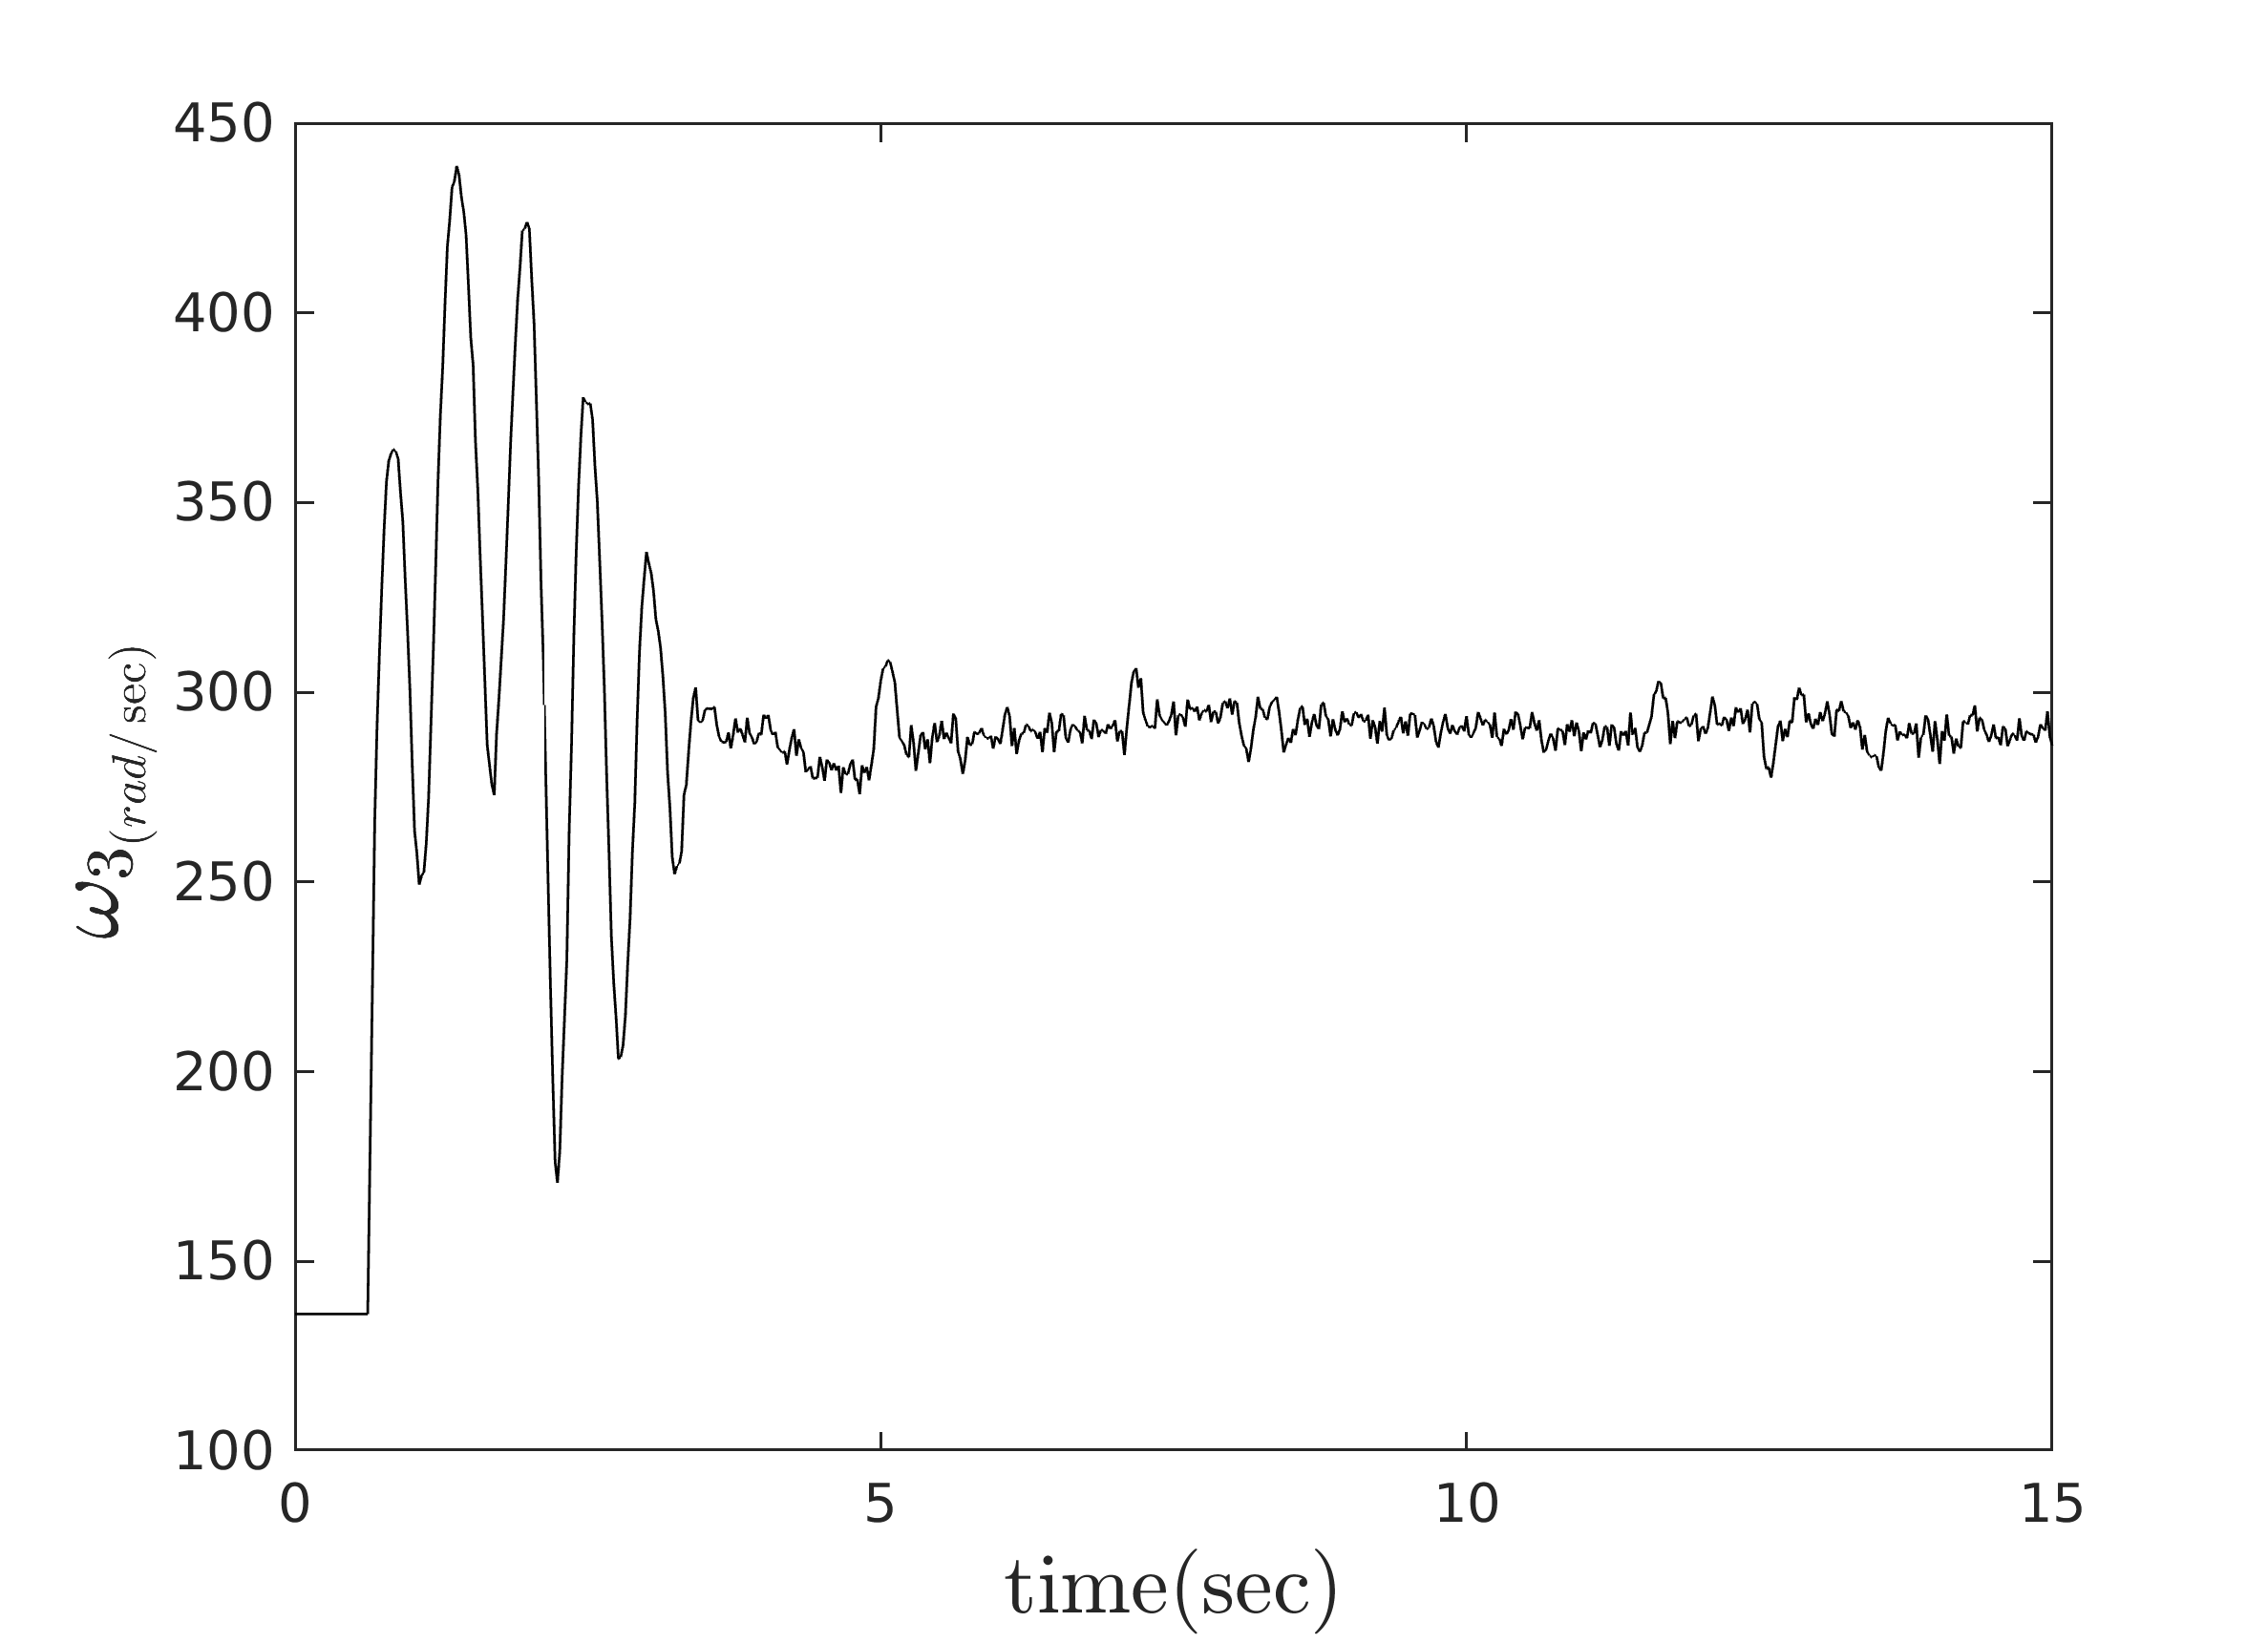
\includegraphics[width=.45\linewidth]{../Figures/MIL/LQIDG/3DOF/lqidg_roll_pitch_Omega_3.png}
	}
	\subfigure[موتور شماره چهار]{
		\centering
		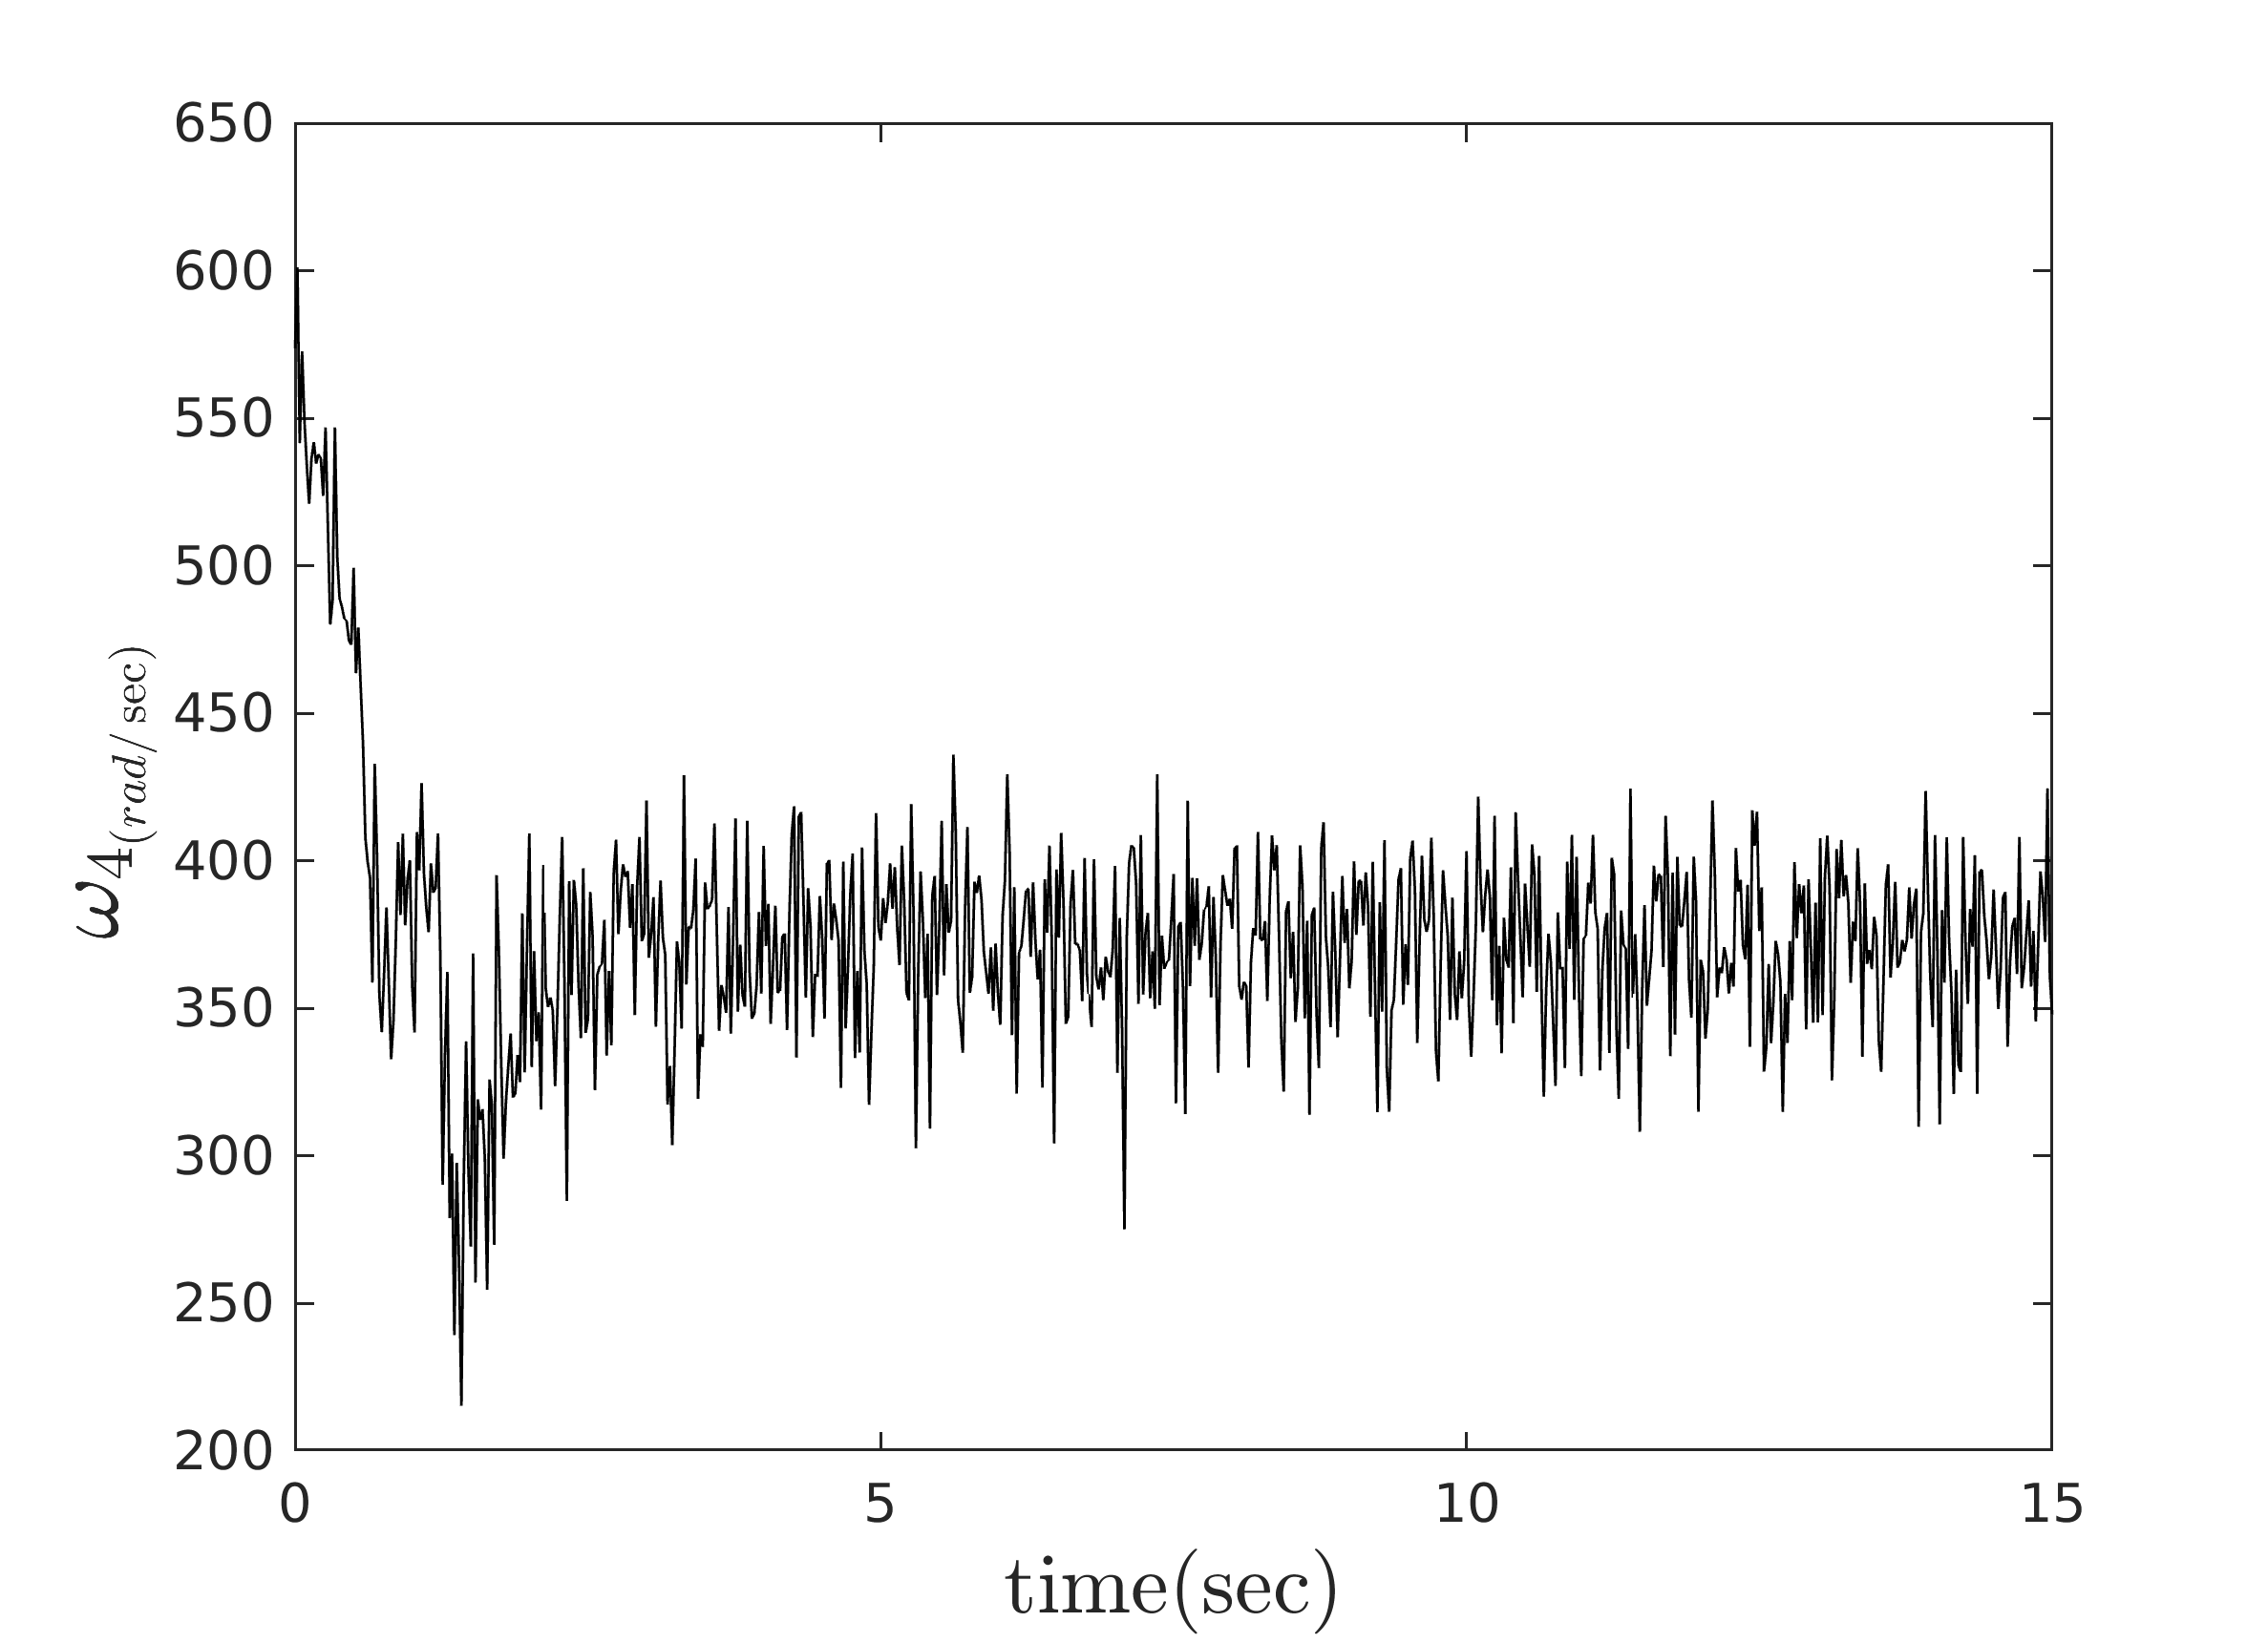
\includegraphics[width=.45\linewidth]{../Figures/MIL/LQIDG/3DOF/lqidg_roll_pitch_Omega_4.png}
	}
	\caption{‫‪فرمان کنترلی موتورها در کنترل وضعیت با حضور نويز اندازه‌گیری}
	\label{3dof_noise_siso}
\end{figure}

\بدون‌تورفتگی همانطور که از شکل
\ref{3dof_noise_siso}
مشخص است، عملکرد کنترل‌کننده \lr{LQDG} در برابر نویز اندازه‌گیری خوب است و خروجی نوسان ندارد.
